\chapter{Heavy flavours} % Main chapter title
\label{Chapter2} % For referencing the chapter elsewhere, use \ref{Chapter1} 

\section{The importance of being heavy}
\label{sec:introChap2}
Hadrons carrying heavy flavour (charm or beauty quarks) 
constitute a powerful probe to study 
the properties of the Quark-Gluon Plasma created in high-energy 
heavy-ion collisions. Heavy quarks are produced in initial hard parton-scattering processes
of the nucleon-nucleon collisions and on short time scales ($\sim$~0.1 and 0.02~fm/$c$ for charm and beauty, respectively) compared 
to the QGP formation time, which is about 0.3-1.5~fm/$c$ at Large Hadron Collider (LHC) energies~\cite{Liu:2012ax}.
Furthermore, in contrast with light quarks and gluons, that can be produced or annihilated 
during QGP evolution, heavy quarks have negligible annihilation 
rate~\cite{BraunMunzinger:2007tn} and secondary "thermal" 
charm and beauty production from processes like $gg \rightarrow c\overline{c}$ is 
expected to be negligible in the QGP~\cite{Zhang:2007dm}, 
unless the initial QGP temperatures happen to be much larger than 
those currently reachable at colliders. Therefore,
heavy quarks preserve their identity when traversing 
the fireball and can be used as a probe
to study the interaction with the medium
 constituents, in particular getting access to the 
transport coefficients of the QGP.\\
There are different ways to experimentally detect hadrons 
containing heavy flavours:
\begin{itemize}
\item full reconstruction of exclusive decay channels, 
like $\DtoKpi$ or $B^0 \rightarrow J/\psi K^0_S$;
\item detection of leptons from heavy-flavour hadron decays, for example 
$D, B \rightarrow e, \mu + X$;
\item selection of semi-inclusive decays, 
for example $J/\psi$ mesons displaced 
from the primary vertex (thus, coming from beauty decay) or $\Lambda_c$ and
$\Xi_c$ reconstruction from $e\, \Lambda$ and $e\, \Xi$ pairs;
\item reconstruction of $c-$ and $b-$jets.
\end{itemize}
\section{Heavy-quark production in pp collisions}
\label{sec:HFpp}
The study of heavy flavours in pp collisions is an 
important benchmark of perturbative QCD calculations. 
The large mass of these quarks acts as a cut off; it prevents 
indeed from divergencies in the calculation that arise
from collinear gluon radiation and that are suppressed 
in case of massive quarks due to the
so-called dead-cone effect~\cite{Dokshitzer:1991fd}. 
For this reason, perturbative calculations are applicable down to low $\pt$ 
as well as for the computation of the total cross-section. 
The two processes responsible for heavy-quark production 
at the leading order in perturbative theory are 
$q \overline{q} \rightarrow Q \overline{Q}$ and $gg \rightarrow Q \overline{Q}$, 
whose corresponding diagrams are
shown in Fig.~\ref{fig:LOdiagrams}. The relative production 
rates for heavy quarks of mass 
$m_1$ and $m_2$ behave, at high energy, as~\cite{Mangano:1997ri}:
\begin{equation}
\begin{aligned}
\frac{\sigma (gg \rightarrow Q_1 \overline{Q}_1)}{\sigma (gg \rightarrow Q_2 \overline{Q}_2)} & \rightarrow 1 - \frac{{\rm log}(m_1^2/m_2^2)}{{\rm log}(s/m_2^2)}, \\
\frac{\sigma (q \overline{q} \rightarrow Q_1 \overline{Q}_1)}{\sigma (q \overline{q} \rightarrow Q_2 \overline{Q}_2)} & \rightarrow 1 - \mathcal{O} (m_1^4/s^2),
\end{aligned}
\end{equation}
hence, at large center-of-mass energy $s$, the 
$q \overline{q} \rightarrow Q \overline{Q}$ process
vanishes more quickly. In the left panel of Fig.~\ref{fig:HQxsecPPcoll}
 the inclusive production cross-section in pp collisions,
as a function of center-of-mass energy, for charm, bottom, 
top quark pairs is shown~\cite{Mangano:1997ri}.
\begin{figure}[!ht]
  \centering
  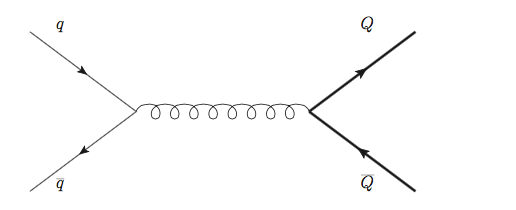
\includegraphics[width=8cm]{FigCap2/Feymann1.png}
  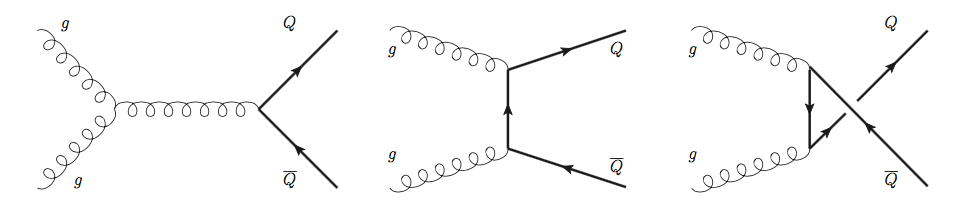
\includegraphics[width=15cm]{FigCap2/Feymann2.png}
  \caption{Leading-order diagrams for heavy-quark pair production.}
  \label{fig:LOdiagrams}
\end{figure}
Analytic calculations that provide a description for inclusive 
heavy-hadron production or their decay products
in pp collisions utilising the collinear factorisation approach 
are FONLL~\cite{Cacciari:1998it,Cacciari:2001td} 
and GM-VFNS~\cite{Kniehl:2004fy}. 
FONLL is a Fixed-Order calculation with Next-to-Leading-Logarithms 
resummation and provides calculations in the full kinematic range 
($\pt \ll m_q, \pt \sim m_q, \pt \gg m_q$),
giving description of bottom and charm production at Tevatron, RHIC and LHC. 
GM-VFNS was originally performed in the massless limit 
and subsequently improved with finite mass terms.
Within both approaches, the single inclusive distribution of a 
heavy-flavour hadron $H_q$ is obtained as a convolution of a
perturbative cross section $d\sigma$ at the partonic level with 
parton distribution functions $f(x, Q^2)$ and non-perturbative 
fragmentation function $D^{NP}_{q->H_q}$.
Possibly a decay function $g^{weak}_{H_q \rightarrow l}$ 
describing, for instance, the hadron weak decay into a lepton can be included:
\begin{equation}
d\sigma_l = f(x, Q^2) \otimes d\sigma_{q} \otimes D^{NP}_{q->H_q} \otimes g^{weak}_{H_q \rightarrow l}.
\end{equation}
The functional form of the non-perturbative fragmentation 
function (FF) $D^{NP}_{q->H_q}$ 
is generally chosen as result of fit on $e^+e^-$ data for 
heavy-hadron production. For example, FONLL uses
a Kartvelishvili et al.~distribution~\cite{Kartvelishvili:1977pi} 
for the FF of bottom quarks:
\begin{equation}
D^{NP}_{b->H_b}= (\alpha +1 )(\alpha +2)z^{\alpha} (1-z),
\end{equation}
where the fragmentation parameter $\alpha$ was chosen as a 
result of the fit on the LEP data concerning production
of a mixture of $b$-hadrons~\cite{Cacciari:2005uk,Heister:2001jg,Abbiendi:2002vt}, 
since no data are available for individual hadrons like $B^0$ or $B^+$.
\begin{figure}[!ht]
  \centering
  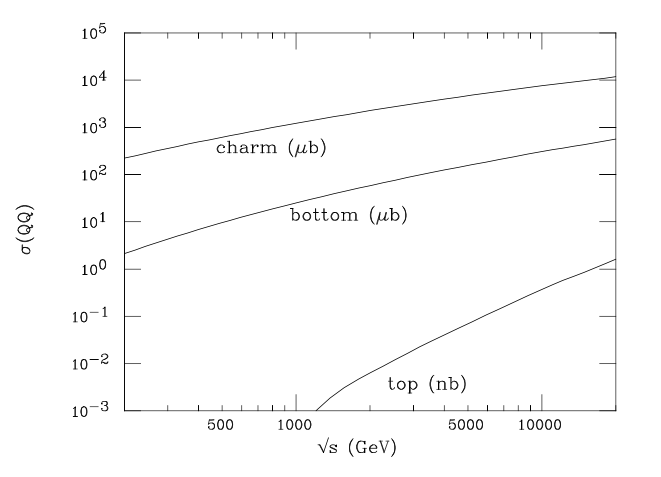
\includegraphics[width=7.6cm]{FigCap2/HQxsecPPcoll.png}
      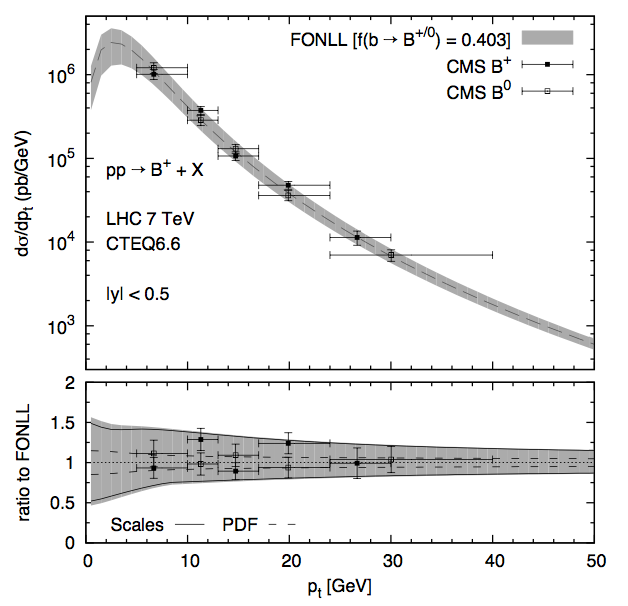
\includegraphics[width=6.4cm]{FigCap2/FONLLBmeson.png}
  \caption{Left: total production cross-sections for charm, bottom and top quark pairs, in pp collisions as a function of the center-of-mass energy~\cite{Mangano:1997ri}. Right: FONLL calculation and systematic uncertainty band~\cite{Cacciari:2012ny} for beauty-hadron production, rescaled to the $|y| <$ 0.5 region, and comparison with CMS data~\cite{Khachatryan:2011mk,Chatrchyan:2011pw}.}
  \label{fig:HQxsecPPcoll}
\end{figure}
For charm quarks, experimental data for individual D-meson species exist.
Since from the theoretical point of view some differencies are 
expected in the quark fragmentation into 
pseudo-scalar ($\Dzero, \Dplus$) and vector ($\Dstar$) mesons, 
one needs to define two different FF. The functional forms used for
the FF of charm quarks in FONLL are taken from~\cite{Cacciari:2003zu}
and have one single non-perturbative parameter
common to the pseudo-scalar and vector FF. This parameter is adjusted on
ALEPH data~\cite{Barate:1999bg} for $\Dstar$ production.
Fig.~\ref{fig:HQxsecPPcoll} (right) shows the CMS measurement 
of $\pt$-differential cross-section for $B^+$ and $B^0$ mesons
as a function of $\pt$ in the rapidity interval $|y| < 0.5$ in pp collision 
at $\sqrt{s} = 7$ TeV~\cite{Khachatryan:2011mk,Chatrchyan:2011pw}, 
compared to FONLL predictions.
The FONLL uncertainty band is obtained from variations of 
renormalisation scale $\mu$ and common factorisation
scale $\mu_f$ as well as of the heavy-quark mass.
Similar comparison, but for charmed hadrons, is shown in Fig.~\ref{fig:CharmXsec} 
for $\Dzero$-meson production
in pp collision at $\sqrt{s} = 7$ TeV measured by 
ALICE~\cite{Acharya:2017jgo}, as a function of $\pt$. FONLL 
predictions are displayed in the left panel and GM-VFNS in the right one. 
Calculations are in agreement with bottom and charm production 
at the LHC, within their
uncertainties. FONLL central values tend to underestimate charm production, 
that systematically lays on the upper edge of FONLL uncertainty band, 
whereas GM-VFNS tends to slightly overestimate the production 
at high $\pt$ but agrees very well at intermediate-low $\pt$. \\



In contrast to FONLL and GM-VFNS, that are based on NLO 
pQCD calculations and are limited to inclusive production
of heavy quarks and mesons, general-purpose Monte Carlo 
generators, such as PYTHIA~\cite{Sjostrand:2006za}, provide a more complete description 
of the final state, including decay kinematics. They simulate the 
final states of high-energy collisions in full detail, including hard and 
soft interactions, parton distributions, initial- and final-state parton 
showers, multiple parton interactions, fragmentation and decay. They contain a large 
list of hard Standard Model and Beyond Standard Model processes, 
which are interfaced with parton emission, different models of hadronisation and particle decays. 
The processes are treated at leading order (LO). The higher order 
calculations are included only in an
approximate approach. However, the next-to-leading order (NLO) 
is needed to compare results with experimental data.
The PYTHIA generator, for example, contains 
theoretical perturbative QCD calculations that are exact only
at leading order, where only the pair creation processes 
$q\overline{q} \rightarrow Q\overline{Q}$ and $gg \rightarrow Q\overline{Q}$
are included. Higher-order contributions at the NLO to account 
for flavour excitation processes like $qQ \rightarrow qQ$, $gQ \rightarrow gQ$
and gluon splitting $g \rightarrow Q\overline{Q}$ are also accounted. 
The cross-section of these processes 
diverges as the transverse momentum of the outgoing quarks of the 
hard interaction ($\pt^{hard}$) goes to zero. 
The divergences can be controlled by a lower cut 
on the value of  $\pt^{hard}$, that has a large influence in the 
heavy-flavour production 
in the low-$\pt$ region, which is of the prime interest for ALICE. 
To compare PYTHIA to data, $\pt^{hard}$ and
other PYTHIA parameters must be tuned to reproduce as well 
as possible NLO predictions.
The first generator of heavy-quark production that did the effort of matching NLO calculations 
with LO calculations was MC@NLO~\cite{Frixione:2002ik}.
It performed a matching to the general-purpose Monte Carlo generator HERWIG~\cite{Corcella:2000bw}, proposing 
a first solution to the otherwise double counting of NLO events, 
by subtracting the approximated NLO cross sections (which were implemented in HERWIG) from the exact NLO cross section.
The NLO calculations for the hard processes in heavy-flavour production are obtained with the 
POWHEG~\cite{Frixione:2007nw} (Positive Weight Hardest Emission Generator) generator,
that interfaces with PYTHIA and HERWIG parton showers. 

\begin{figure}[!ht]
  \centering
  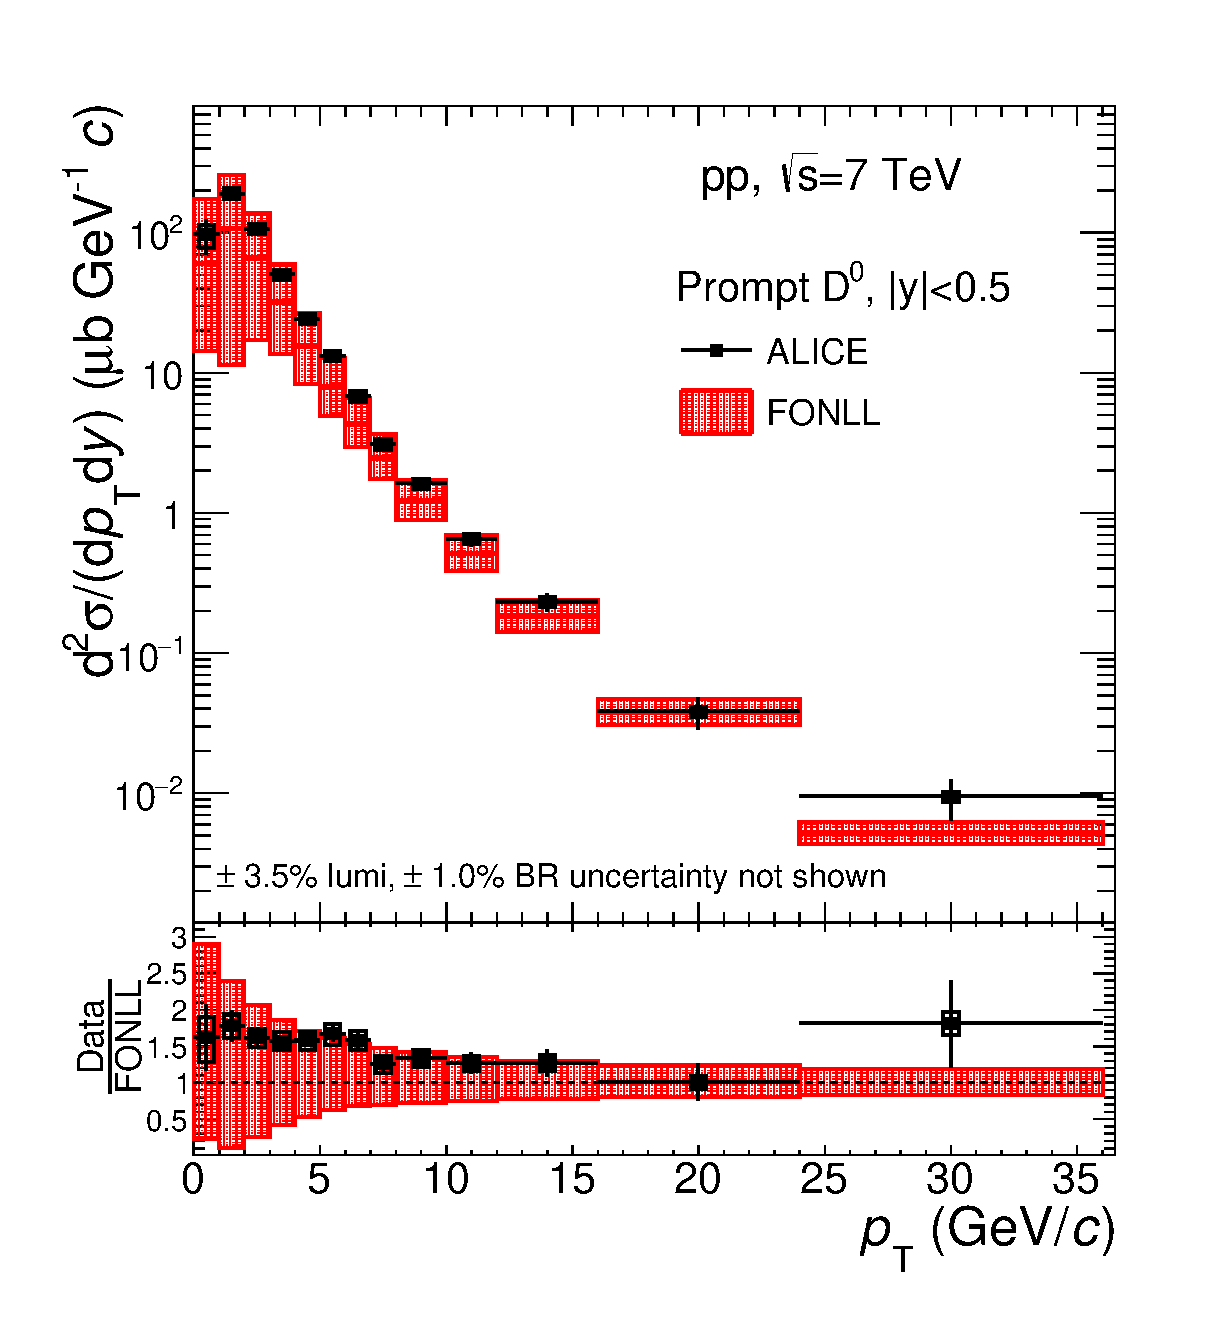
\includegraphics[width=7cm]{FigCap2/DzeroppCrossSecVsFONLLAndRatio.eps}
  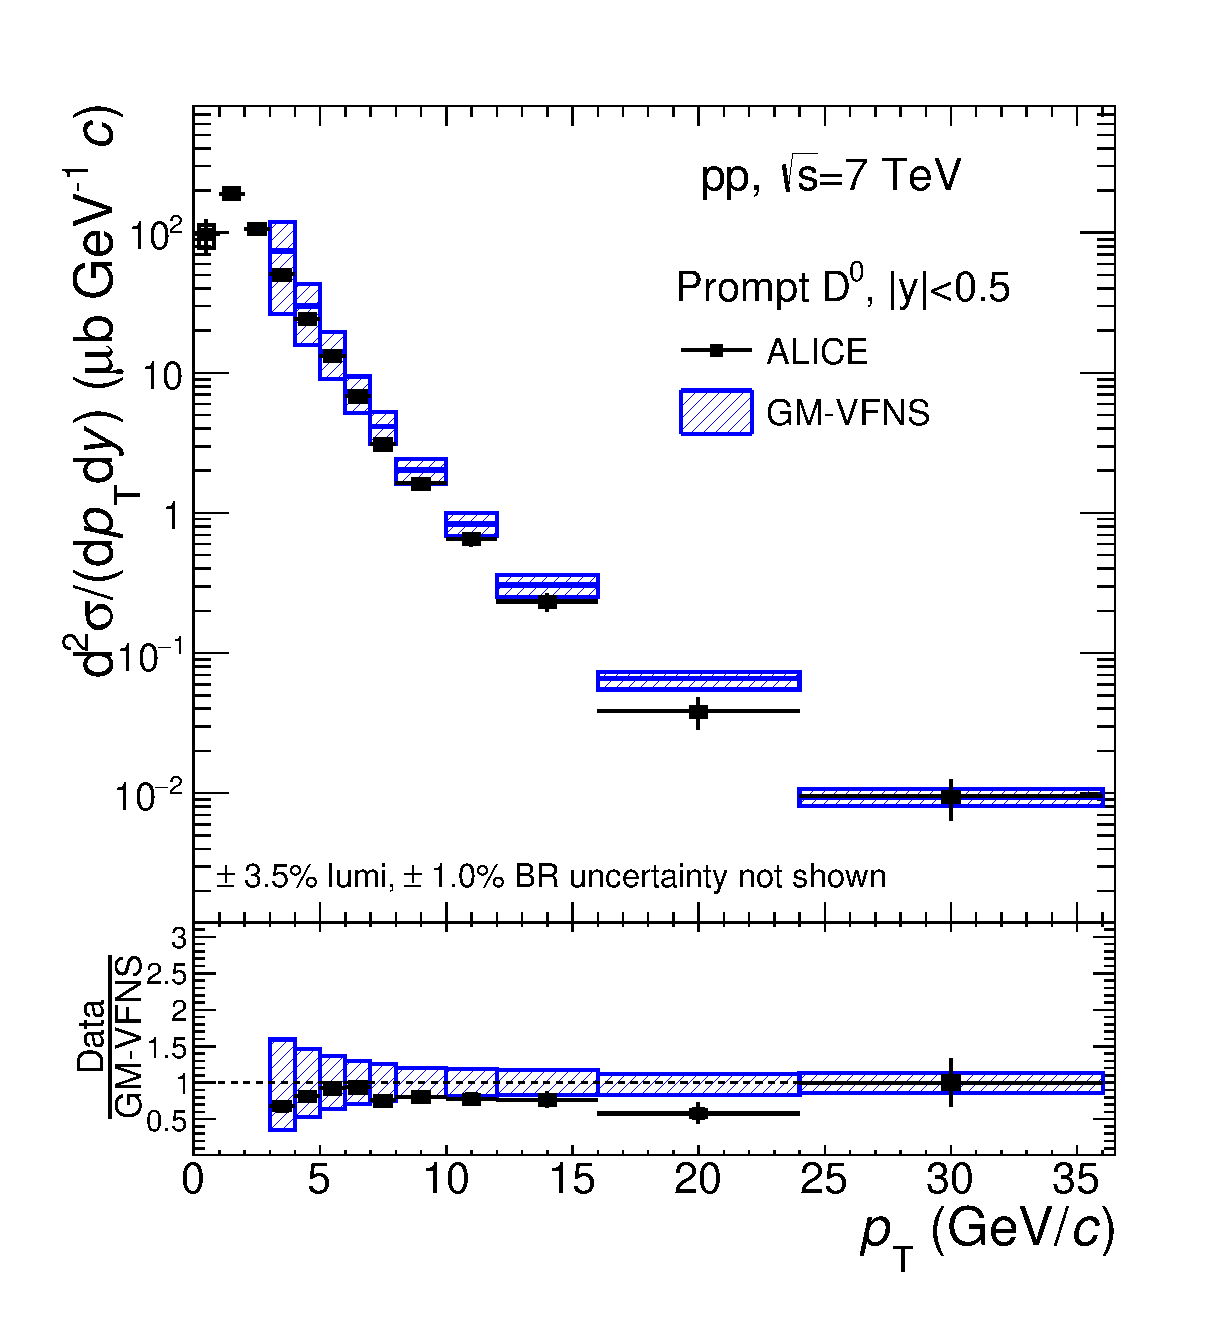
\includegraphics[width=7cm]{FigCap2/DzeroppCrossSecVsGMVFNSAndRatio.eps}
  \caption{$\pt$-differential production cross section of prompt $\Dzero$ mesons with $|y| < $ 0.5 in the interval $0 < \pt < 36 ~\Gevc$, in pp collisions at $\sqrt{s} = 7$ TeV~\cite{Acharya:2017jgo}. The cross section is compared to pQCD calculations: FONLL~\cite{Cacciari:1998it,Cacciari:2001td} (left panel) and GM-VFNS~\cite{Kniehl:2004fy} (right panel).}
  \label{fig:CharmXsec}
\end{figure}

\section{Heavy quarks in p-A collisions}
\label{sec:HFpA}
\subsection{Cold nuclear matter effects}
\label{sec:CNM}
The importance of studying heavy-flavour production in p-A collisions relies on the possibility to
characterise a class of phenomena that are expected to break the binary scaling in 
nucleus-nucleus collisions but are not a consequence of the presence of a 
deconfined plasma. Such effects can in fact be present both in p-A and in A-A collisions and
their origin is mainly related to modification of the PDFs for nucleons bound in nuclei and
multiple soft scatterings of the partons in the nuclei prior to the
hard interaction energy loss in cold nuclear matter. 
They are usually called Cold Nuclear Matter (CNM) effects and
can affect the partons that undergo the hard 
scattering process (initial-state effects) as well as
the produced heavy quarks and hadrons (final-state effects).
Furthermore, recent interest in p-A collisions
is focused on revealing possible effects that could indicate the 
formation of a QGP droplet in small collision systems~\cite{Beraudo:2015wsd,Bozek:2014era,Bzdak:2013zma}.

\subsection{Nuclear Parton Distribution Functions}
\label{sec:nPDFs}
One can quantify the nuclear modification of the parton distribution function via the ratio:
\begin{equation}
\label{eq:RA}
R_i^A(x,Q^2) = f_{i/A}(x,Q^2) / f_{i/p}(x,Q^2)
\end{equation}
\begin{figure}[!ht]
  \centering
  \includegraphics[width=.49\textwidth]{FigCap2/RvEPPS16.png}
  \includegraphics[width=.49\textwidth]{FigCap2/RsEPPS16.png}
  \includegraphics[width=.49\textwidth]{FigCap2/RgEPPS16.png}
  \caption{The nuclear modifications (Eq.~\ref{eq:RA}) in a Pb nucleus $R_i^A(x,Q^2)$ for three different flavours as given by the EPS09~\cite{Sassot:2009sh}, EPPS16~\cite{Eskola:2016oht} and DSSZ~\cite{deFlorian:2011fp} nPDF parameterisations.}
  \label{fig:nPDF}
\end{figure}
where $f_{i/A}(x,Q^2)$ and $f_{i/p}(x,Q^2)$ are the parton distribution functions in the 
nucleus and in the proton respectively, and the variable $x$ represents the fraction of 
the nucleon momentum carried by a parton. Figure~\ref{fig:nPDF} 
shows the ratios $R_i^A(x,Q^2)$ for the valence quarks, sea quarks and 
gluons inside a Pb nucleus as obtained from global DGLAP 
calculations with leading-order EPS09LO~\cite{Eskola:2009uj} and next-to-leading order 
EPPS16~\cite{Eskola:2016oht} and DSSZ~\cite{deFlorian:2011fp}
parameterisations of the nuclear PDFs which are tuned on measurements
of DIS, Drell-Yan and hadron and dijet production in p-A collisions. 
In general, four different regions are visible in the trend of $R_i^A(x,Q^2)$ versus $x$,
which correspond to four $x$-regimes in which different 
effects influence the PDFs of bound nucleons:
\begin{itemize}
\item {\bf Fermi motion:} this effect is due to the 
thermal momentum that nucleons have inside the nucleus. 
Thus the structure function $F^A_2(x)$ of the bound nucleons
is the convolution of the structure function of the free nucleon 
$F^N_2(x/z)$ (where $z$ is the momentum fraction
of the nucleons times the atomic number of the nucleus) 
with the momentum distribution
of nucleons $f_N(z)$ inside the nucleus: 
$F^A_2(x) = \int_x^A dz f_N(z) F_2^N(x/z)$.
This is the dominant effect for $x > 0.7$.
\item {\bf EMC effect:} first observed in 1982 by the EMC collaboration~\cite{Aubert:1983xm},
this effect appears as $R_i^A(x,Q^2)<1$, especially affecting the region 
of valence quarks $0.2 < x < 1$. Figure~\ref{fig:EMC} shows the ratio of the structure functions 
of iron $F^{iron}_2(x)$ and deuterium $F^D_2(x)$, that one would expect to be at 1 (except for 
some corrections at high $x$ from Fermi motion). From further
experimental investigations, it was clear that the effect is almost independent from the 
squared momentum transfer, it increases with nuclear mass 
number A and scales approximately with the average nuclear density. 
Many phenomenological models tried to explain such behaviour. 
In the $Q^2$-rescaling models, 
quarks in nuclei move in a larger confinement volume and, 
because of the uncertainty principle, 
they carry less momentum than quarks in free nucleons. 
Some models proposed that 
quarks in nuclei move in quark bags with $n$ quarks, 
other proposed an enhancement 
of pion-cloud effects and a nuclear pionic field, 
but no models so far are universally accepted. 
\iffalse
 In 2009 other pieces of information were added with the
discovery of a strong correlation between the slope of the ratio $R_i^A(x,Q^2)$ in 
the region of EMC effect and the magnitude of the scaling plateau 
at $x > 1$ (see Fig.~\ref{fig:EMC}, right panel)~\cite{Seely:2009gt}.
\fi
\item {\bf Nuclear shadowing and anti-shadowing:} a second depletion region
is observed in the ratio of parton distribution functions $f_{i/A}(x,Q^2) / f_{i/p}(x,Q^2)$ 
at very low $x<0.01$ (typical region of sea quarks). This is commonly denoted 
by shadowing region and is accompanied by
an anti-shadowing region at $0.01 < x < 0.2$ in which the ratio $R_i^A(x,Q^2)$
is above unity.~Different models were
proposed to explain the nuclear shadowing. Some models are based on virtual 
photon fluctuations into vector meson states (GVMD); others
invoke superposition ad fusion of partons of different nucleons at very low $x$, that should deplete the 
region, thus favouring the population of the anti-shadowing region.

\end{itemize}


\begin{figure}[!ht]
  \centering
  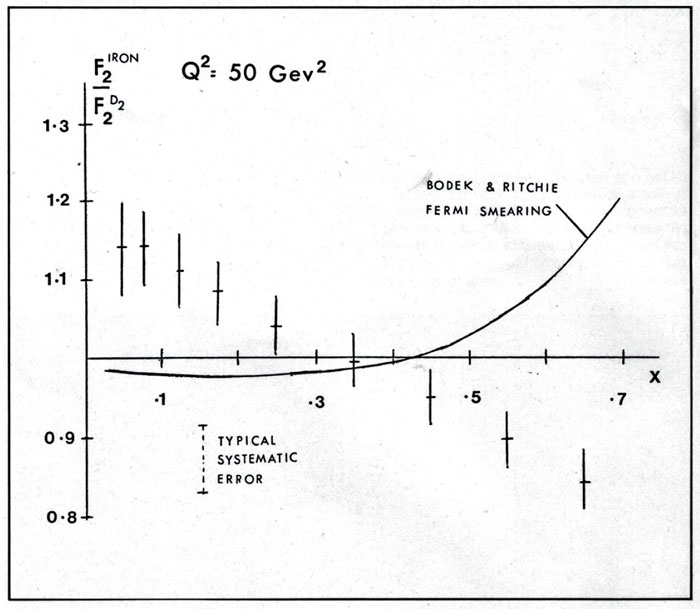
\includegraphics[width=6cm]{FigCap2/EMC.png}
%  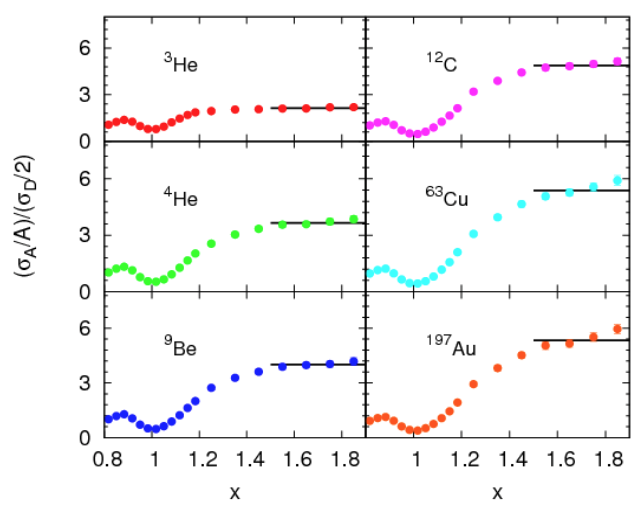
\includegraphics[width=7.5cm]{FigCap2/EMC2.png}
  \caption{Ratio of iron $F^{iron}_2(x)$ and deuterium $F^D_2(x)$ structure function as a function of Bjorken-$x$~\cite{Aubert:1983xm}.% Right: ratio of nucleus $F^{A}_2(x)$ and deuterium $F^D_2(x)$ for different nuclei as a function of Bjorken-$x$~\cite{Seely:2009gt}.
  }
  \label{fig:EMC}
\end{figure}



An other CNM effect is the so-called Cronin Effect~\cite{Cronin:1974zm}, 
discovered in the '70s at FermiLab. It consists in an observed 
enhancement in the nuclear modification factor for $\pt$ 
values between 2 and 5 $\Gevc$. This is commonly understood as due to 
the fact that, in p-A collisions, the 
partons of the projectile nucleon undergo several elastic 
scatterings with the partons of the target nucleus before the hard scattering process 
occurs. The multiple scatterings give the parton an extra 
momentum component in the transverse plane ($k_{\rm T}$ broadening), 
which causes a broadening of the $\pt$ spectra of the heavy 
quarks produced in the hard scattering processes,  
resulting in an enhancement of the nuclear modification factor at 
low and intermediate $\pt$. Going towards 
larger values of transverse momentum, the extra-$k_{\rm T}$ 
from the elastic collisions becomes negligible and the nuclear 
modification factor gets close to unity.\\
%The x regime relevant for charm production at the LHC ($\sim 10^{-4}$ ) is about 2 orders of magnitude lower than at RHIC and 3 orders of magnitude lower than at the SPS [43]. In this region with low x-values, modifications of the nuclear PDFs are mainly related to the shadowing effect.
\begin{figure}[!ht]
  \centering
  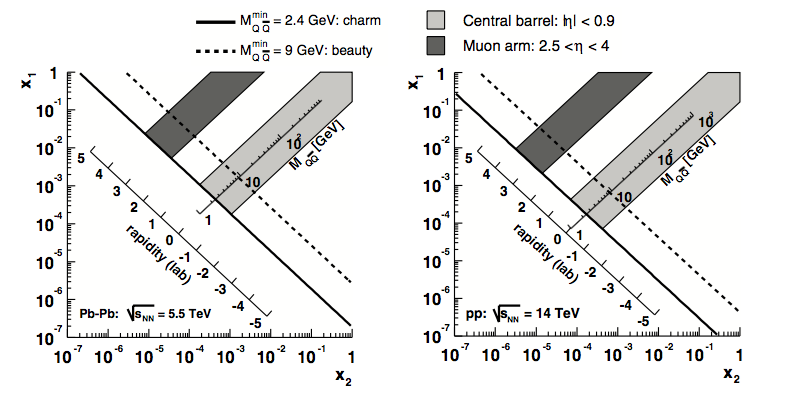
\includegraphics[width=15cm]{FigCap2/xBjork.png}
  \caption{ALICE acceptance in the ($x_1, x_2$) plane for heavy flavours in Pb-Pb at $\sNN = 5$ TeV on the left panel and pp collisions at $\sqrt{s} = 14$ TeV on the right~\cite{Alessandro:2006yt}. }
  \label{fig:xBjork}
\end{figure}



It is important to understand which are the ranges of Bjorken $x$
at play when producing $c\overline{c}$ and $b\overline{b}$ pairs at the LHC. 
The probed $x$ value depends on the center-of-mass energy
of the collision, on the invariant mass $M_{Q\overline{Q}}$ of the 
$Q\overline{Q}$ pair produced in the hard scattering
and on its rapidity $y_{Q\overline{Q}}$. Under the hypothesis 
that the transverse momentum of the parton 
in the nucleon is negligible, the four-momenta of the two 
incoming gluons are $(x_1,0,0,x_1)\cdot(Z_1/A_1)\sqrt{s_{\rm pp}}/2$
and $(x_2,0,0,-x_2)\cdot(Z_2/A_2)\sqrt{s_{\rm pp}}/2$, where 
$x_1$ and $x_2$ are the momentum fractions 
carried by the gluons, and $\sqrt{s_{\rm pp}}$ is the c.m.s. energy for pp collisions.
The c.m.s $\sNN$ energy of nucleon-nucleon collisions is obtainable as $\sNN=Z/A\sqrt{s_{\rm pp}}$.
The square of the invariant mass of the produced $Q\overline{Q}$ pair is given by:
\begin{equation}
\label{eq:Mqq}
M_{Q\overline{Q}}^2 =  x_1 x_2 s_{\rm NN} = x_1 \frac{Z_1}{A_1} x_2 \frac{Z_2}{A_2} s_{\rm pp},
\end{equation}
and the rapidity in the laboratory is:
\begin{equation}
\label{eq:yqq}
y_{Q\overline{Q}} = \frac{1}{2} {\rm ln} {\Big [ } \frac{E +p_z}{E-p_z}  {\Big ] }= \frac{1}{2} {\rm ln} {\Big [ } \frac{x_1}{x_2} \cdot \frac{Z_1 A_2}{Z_2 A_1} {\Big ] }.    
\end{equation}
From Eq.~\ref{eq:Mqq} and~\ref{eq:yqq} and for a symmetric colliding system $(A_1 = A_2, Z_1 = Z_2)$
one obtains:
\begin{equation}
\label{eq:x1x2}
x_1 = \frac{M_{Q\overline{Q}}}{\sqrt{s_{\rm NN}}} {\rm exp} (+y_{Q\overline{Q}} ), \; \; \; \; \; \;
x_2 = \frac{M_{Q\overline{Q}}}{\sqrt{s_{\rm NN}}} {\rm exp} (-y_{Q\overline{Q}} ). 
\end{equation}\\




Because of its lower mass, charm allows to probe lower $x$ values than beauty. 
The $x$ regime relevant for charm production at the LHC ($\approx 10^{-4}$) is about 
2 orders of magnitude lower than at RHIC and 3 orders of magnitude lower than at the SPS.
Measurements of charm and beauty particles in the forward (or backward) rapidity region ($|y| \sim 4 $) 
gives access to $x$ regimes about 2 orders of magnitude lower, down to $x \approx 10^{-6}$.
Figure~\ref{fig:xBjork}~\cite{Alessandro:2006yt} shows the ($x_1, x_2$) 
plane for charm and bottom production at the LHC
covered by the ALICE acceptance, for Pb-Pb
collisions at $\sNN = 5$ TeV on the left panel and pp collisions 
at $\sqrt{s} = 14$ TeV on the right.
The shadowed regions correspond to the rapidity region covered 
by the ALICE central barrel ($|\eta| < 0.9$) and by the 
muon arm ($2.5 < \eta < 4$).
The points with equal invariant mass (solid and dashed lines for $c\overline{c}$ and $b\overline{b}$ pairs respectively) 
lie on hyperbolae (straight lines in the log-log scale).\\


\subsection{Experimental results in p-A collisions}
\label{sec:HFresultspA}
The nuclear modification of the PDFs can significantly affect final hadrons yields,
especially at low $\pt$ due to shadowing, which is the most relevant effect at LHC energies.
One can define the nuclear modification factor for p-Pb collisions as:
\begin{equation}
R_{\rm pPb} = \frac{1}{A}\frac{d^2\sigma_{pPb}^{\rm prompt D}/d\pt dy}{d^2\sigma_{pp}^{\rm prompt D}/d\pt dy},
\end{equation}
where A is the Pb mass number $A = 208$. \\
\begin{figure}[!ht]
  \centering
  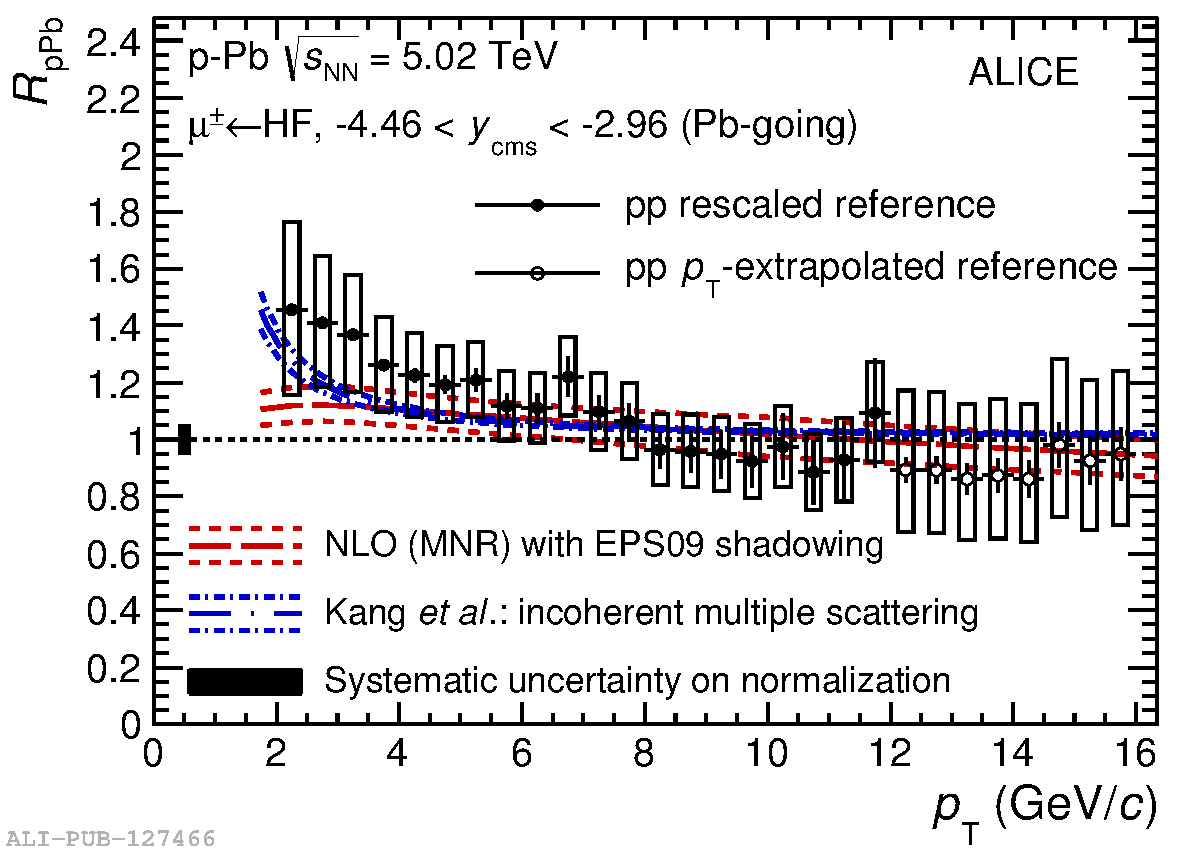
\includegraphics[width=7cm]{FigCap2/2017-Feb-05-Fig2b.pdf}
  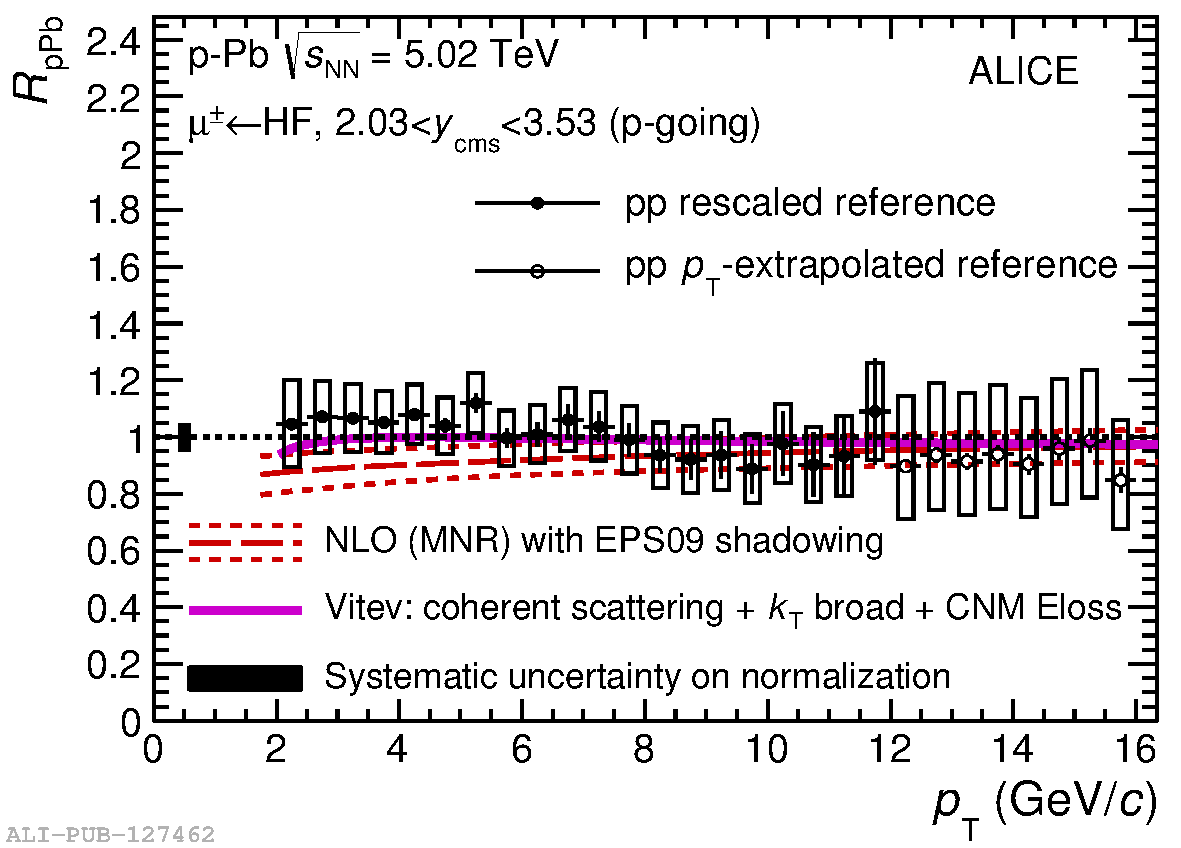
\includegraphics[width=7cm]{FigCap2/2017-Feb-05-Fig2a.pdf}
  \caption{Nuclear modification factor of muons from heavy-flavour hadron decays as a function of $\pt$ for p-Pb collisions at $\sNN = 5.02$ TeV at backward rapidity ($-4.46 < y_{\rm cms} < -2.96$, left) and forward rapidity ($2.03 < y_{\rm cms} < 3.53$, right)~\cite{Acharya:2017hdv} compared to model predictions~\cite{Kang:2014hha,Mangano:1991jk}. }
  \label{fig:muons}
\end{figure}
\begin{figure}[!ht]
  \centering
    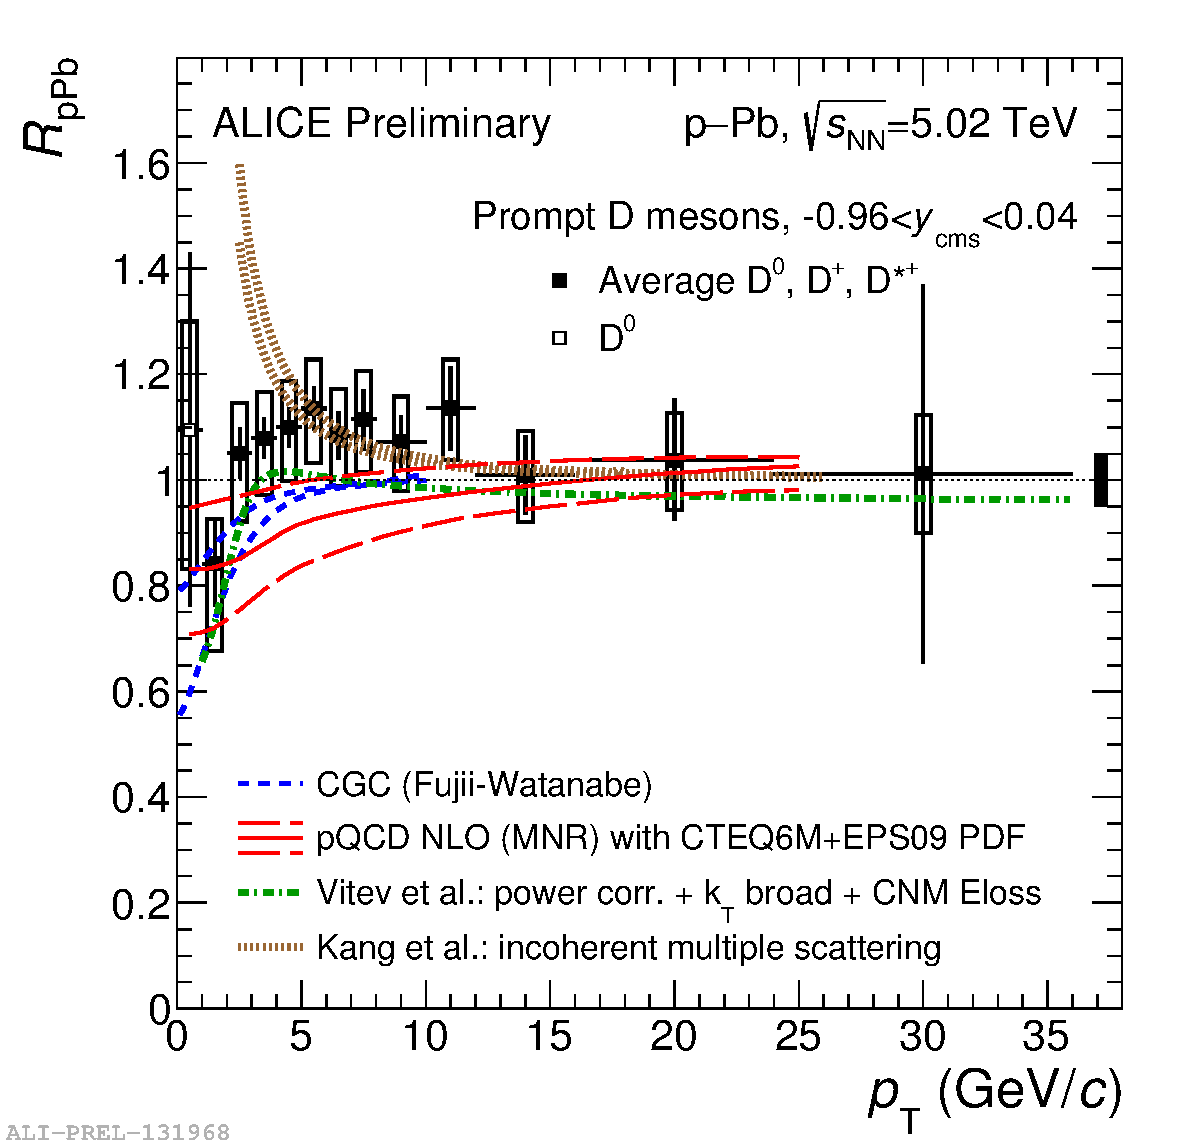
\includegraphics[width=7cm]{FigCap2/2017-Jul-05-pPbWithModelsCNM.pdf}
    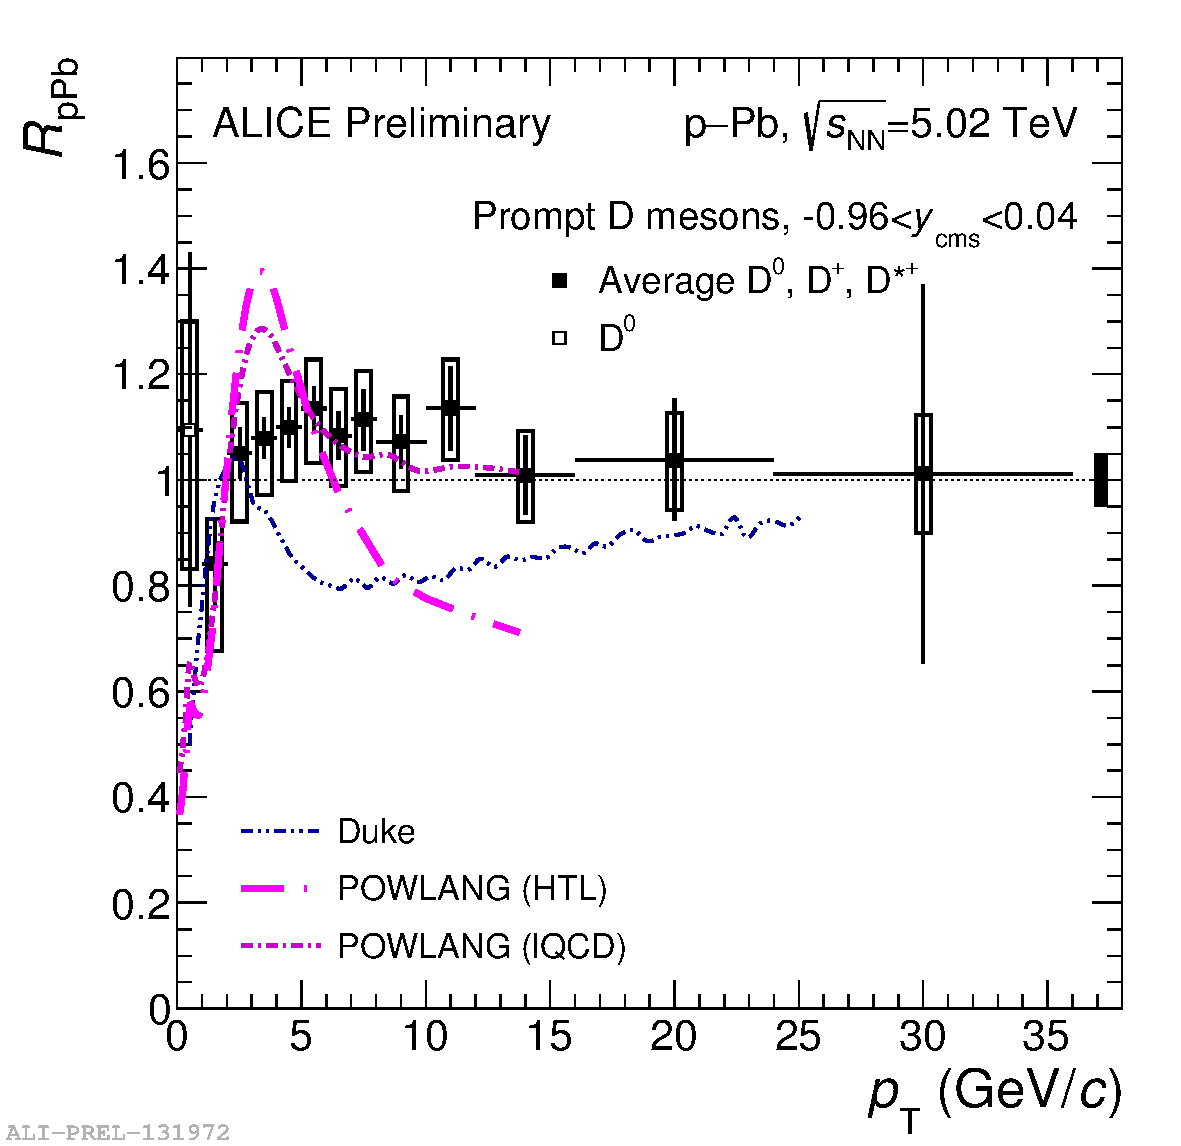
\includegraphics[width=7cm]{FigCap2/pPbWithModelsMedium.pdf}
  \caption{Left: nuclear modification factor $R_{\rm pPb}$ of prompt D mesons in p-Pb collisions at $\sNN = 5.02$ TeV. Data are compared with results of theoretical calculations including only CNM effects~\cite{Fujii:2017rqa,Cacciari:2012ny,Eskola:2016oht,Sharma:2009hn,Kang:2014hha}. Right: the results of the Duke~\cite{Xu:2015iha} and POWLANG~\cite{Beraudo:2015wsd} transport models are compared with the measured D-meson $\RpPb$.}
  \label{fig:RpA}
\end{figure}


ALICE measured the $\pt$-differential nuclear modification factor 
$R_{\rm pPb}$ of muons from heavy-flavour hadron decays in p-Pb collisions at $\sNN = 5.02$ TeV
at forward and backward rapidity~\cite{Acharya:2017hdv} (Fig.~\ref{fig:muons}).
At backward rapidity, the Bjorken-$x$ values are expected to vary from about 10$^{-3}$ to 10$^{-1}$, 
while at forward rapidity they are located in the range from about 5$\cdot 10^{-6}$ to $10^{-2}$.
While at forward rapidity muon $R_{\rm pPb}$ is compatible 
with unity in the full $\pt$ range ($2 <\pt < 16 \, \Gevc$) in which the 
measurement was carried out, 
at backward rapidity, it is larger than unity at low $\pt$ with a maximum 
deviation of $R_{\rm pPb}=1$ of 2.2$\sigma$ of the combined statistical and 
systematic uncertainties in the interval $2.5 < \pt < 3.5 \;\Gevc$. 
At higher $\pt$, it is compatible with unity. The results indicate
that CNM effects are small and that the strong suppression of the
yields of muons from heavy-flavour hadron decays observed in the
10\% most central Pb-Pb collisions~\cite{Abelev:2012qh} should result from final-state
effects, i.e. the heavy-quark in-medium energy loss. 
ALICE also measured the $R_{\rm pPb}$ of prompt 
D mesons in p-Pb collisions at $\sNN = 5.02$ TeV
as a function of $\pt$ and the results are shown in 
Fig.~\ref{fig:RpA} (left panel)~\cite{ALICEPAS2017008}. 
Data are compared to theoretical models that include CNM effects: 
a calculation based on the Color Glass Condensate
formalism~\cite{Fujii:2013yja,Fujii:2017rqa}, a FONLL 
calculation~\cite{Cacciari:2012ny} with CTEQ6M PDFs~\cite{Pumplin:2002vw} 
and EPPS16 NLO nuclear modification~\cite{Eskola:2016oht}, 
a LO pQCD calculation with intrinsic $k_{\rm T}$ broadening, 
nuclear shadowing and energy loss of the charm quarks 
in cold nuclear matter (Vitev et al.)~\cite{Sharma:2009hn}, 
and a higher-twist calculation based on incoherent multiple 
scatterings (Kang et al.)~\cite{Kang:2014hha}. 
The three former calculations describe the data within 
uncertainties in the entire $\pt$ range, although for the CGC 
calculation the compatibility with the data 
in 3-12 $\Gevc$ is at the limit of the uncertainties of the data 
and of the calculations. The calculation by Kang et al., which has 
a different trend with respect to the others, is disfavoured by the 
data for $\pt<3$--$4~\gev/c$.
CNM effects are expected to be largest for small $\pt$, where, in 
addition, the predictions of the different theoretical approaches differ 
and the statistical uncertainty of the present measurement for the 
lowest $\pt$ interval is about 30\% and does not 
discriminate the different models.
In the right-hand panel of Fig.~\ref{fig:RpA}, the data are 
compared with the results of two transport model 
calculations, Duke~\cite{Xu:2015iha} and 
POWLANG~\cite{Beraudo:2015wsd}, both of them assuming that a 
Quark--Gluon Plasma is formed in p--Pb collisions.
Both models are based on the Langevin approach for the transport of heavy 
quarks through an expanding deconfined medium described by relativistic viscous 
hydrodynamics. In both the Duke and POWLANG results the D-meson nuclear modification
factor shows a structure with a 
maximum at $\pt \approx 2.5~\Gevc$ and $\pt \approx 3-4~\Gevc$ respectively, followed by a moderate 
($<20$-30\%) suppression at higher $\pt$,
resulting from the interplay of CNM effects and interactions of charm quarks with the
radially expanding medium.
The trend predicted by these models is disfavoured by the data, which in particular 
disfavour a suppression 
larger than 10-15\% in the interval $3<\pt<12~\Gevc$.\\
\begin{figure}[!ht]
  \centering
    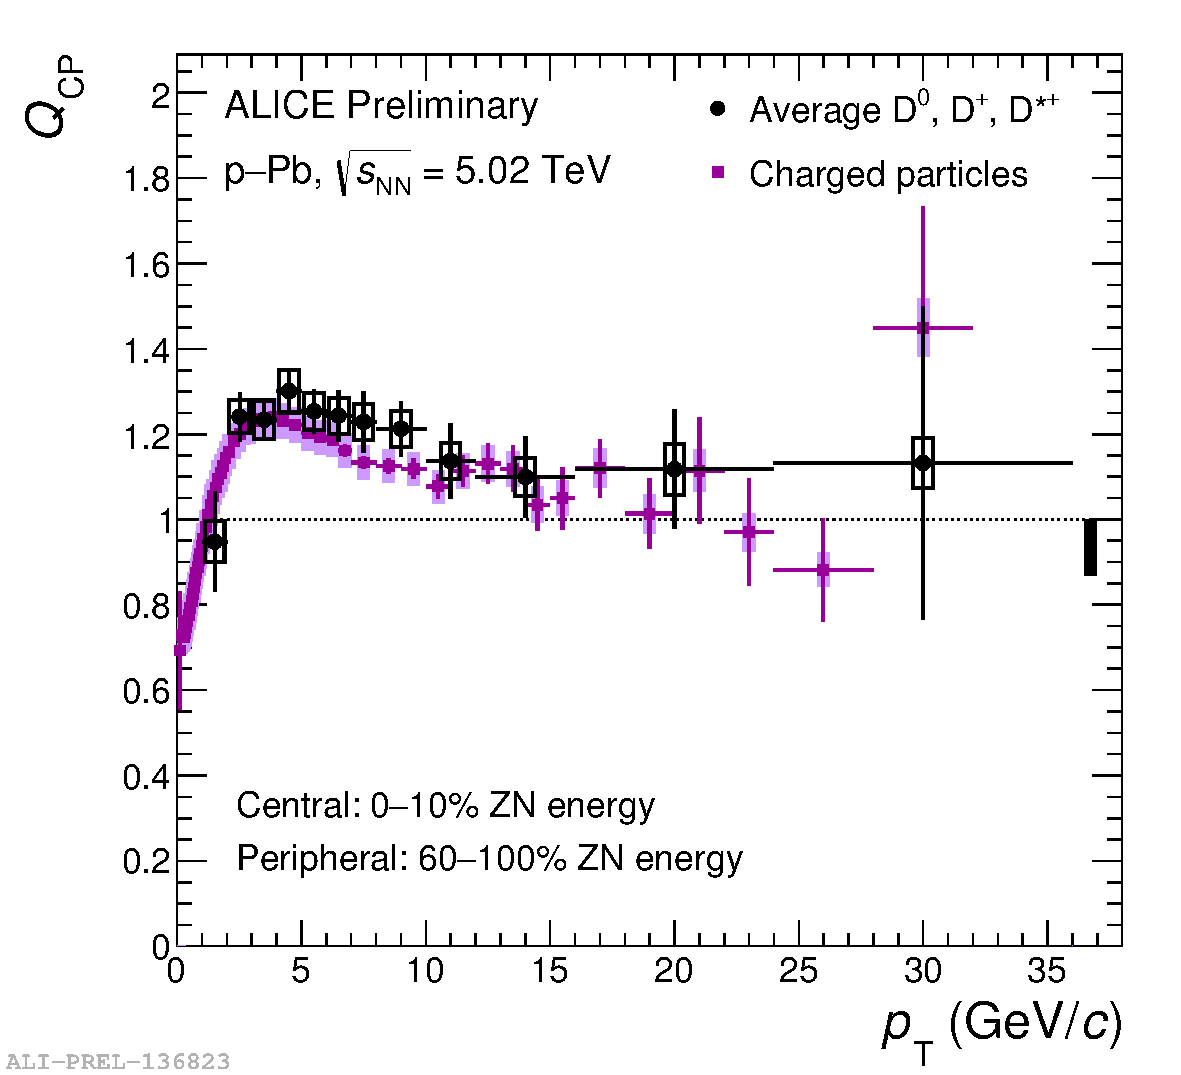
\includegraphics[width=8cm]{FigCap2/2017-Sep-12-QCP-Daverage-ChargedHadrons.pdf}
  \caption{D-meson (black) and charged-particle (magenta) central-to-peripheral nuclear modification factor~\cite{ALICEPAS2017008}.}
  \label{fig:QCP}
\end{figure}




The nuclear modification factor in p-Pb collisions can be also measured in given centrality classes.
Its definition is:
\begin{equation}
Q_{\rm pPb}^{\rm mult} = \frac{({\rm d}^2 N/{\rm d} \pt {\rm d} y)^{\rm mult}_{\rm pPb}}{\langle T_{\rm pPb} \rangle ^{\rm mult}({\rm d}^2 \sigma_{pp}/{\rm d} \pt {\rm d} y)},
\end{equation}
where $({\rm d}^2 N/{\rm d} \pt {\rm d} y)^{\rm mult}_{\rm pPb}$ 
is the yield of a given species in p-Pb collisions 
in a given centrality class, and $\langle T_{\rm pPb} \rangle ^{\rm mult}$ is the average nuclear 
overlap function in the same centrality class.
In order to achieve better precision on the yields, the ratio of the nuclear 
modification factor in central to peripheral events, $Q_{\rm CP}$, 
can be defined as:
\begin{equation}
Q_{\rm CP} = \frac{({\rm d}^2 N/{\rm d} \pt {\rm d} y)^{\rm central}_{\rm pPb}/ \langle T_{\rm pPb} \rangle^{\rm central}}{({\rm d}^2 N/{\rm d} \pt {\rm d} y)^{\rm peripheral}_{\rm pPb}/ \langle T_{\rm pPb} \rangle^{\rm peripheral}}.
\label{eq:QCP}
\end{equation}
The $Q_{\rm CP}$ of D mesons in the 0-10\% and 60-80\% 
centrality classes was measured by 
ALICE~\cite{ALICEPAS2017008} (Fig.~\ref{fig:QCP}) 
and it increases in the interval 1-4 $\Gevc$, 
up to values of about 1.25 and then tends to decrease. The 
average value of the D-meson $Q_{\rm CP}$ 
in the interval $3 < \pt < 8 \; \Gevc$ is larger than unity by 1.5 
standard deviations of the combined statistical and systematic uncertainty.
It is an open question whether the observed bump of $Q_{\rm CP}$, whose magnitude is similar 
for D mesons and charged particles, is related to initial state effects 
or to collectivity effects in the final state.
\iffalse
\begin{figure}[!ht]
  \centering
  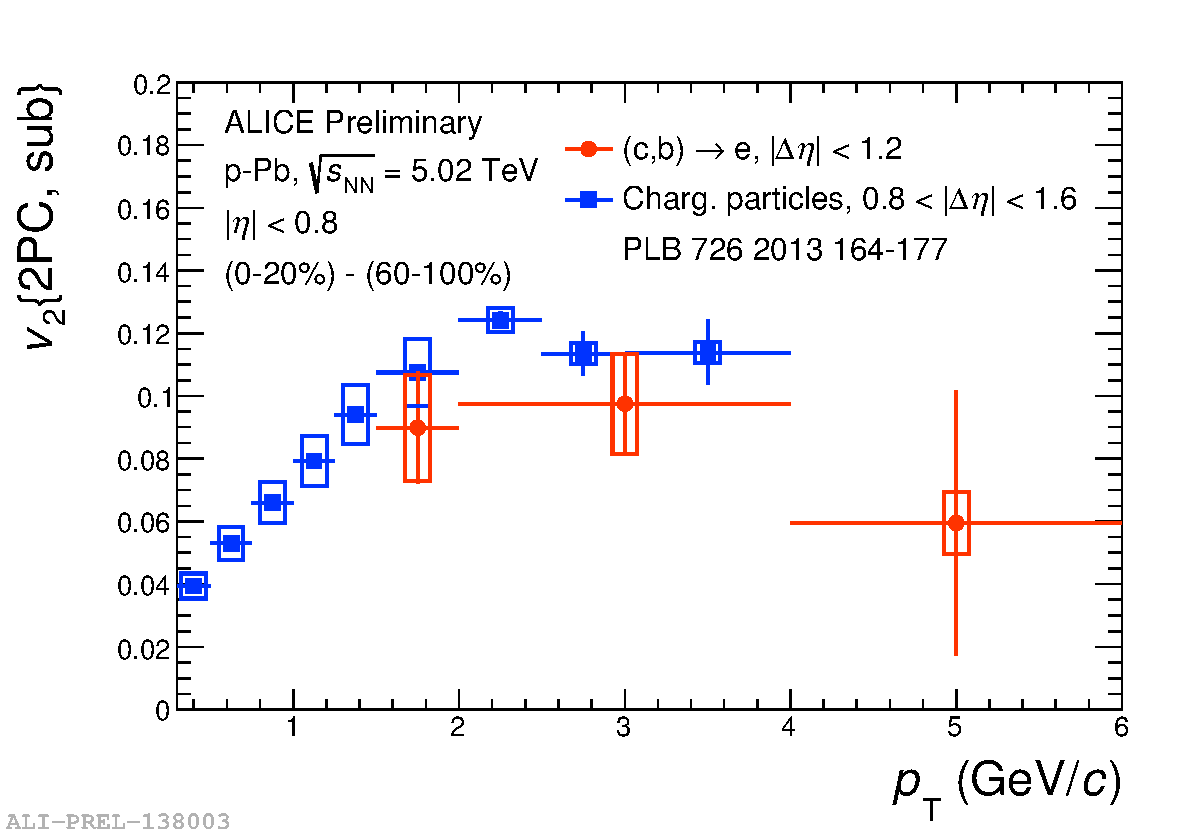
\includegraphics[width=7cm]{FigCap2/v2HFE.pdf}
  \caption{~\cite{Acharya:2017hdv}}
  \label{fig:}
\end{figure}
\fi
\section{Heavy quarks in A-A collisions}
\label{sec:HFEnLossinAA}
High-momentum partons traversing the QGP are expected 
to lose energy because of interactions 
with the medium constituents. One of the experimental observables 
used for the study of energy loss is the 
nuclear modification factor, defined in Sec.~\ref{sec:JetQuenching}. 
The possibility to disentangle
effects of cold nuclear matter from the ones related to in-medium 
energy loss paves the way to characterise the 
hot and dense medium properties. In fact, the magnitude of energy lost in the medium is
determined by the properties of the fireball like the transport coefficients,
that encode the momentum transfers with the medium, or the mean free 
path, closely related to the medium density $\rho$
and the cross section $\sigma$ of the parton-medium interaction. 
A colour charge can lose energy in a plasma at a temperature $T$ by two mechanisms: 
radiative and collisional energy losses, which originate, respectively, from elastic
and inelastic interactions with the medium constituents.
\subsection{Collisional processes}
\label{sec:coll}
Collisional processes are $2 \rightarrow 2$ elastic scatterings off thermal 
gluons (Fig.~\ref{fig:LoopCollScatt}, first to third diagrams) and quarks 
(Fig.~\ref{fig:LoopCollScatt}, fourth diagram). It is possible to calculate,
 in the limit $E \gg M^2/T$, the heavy-quark collisional energy loss 
 ${\rm d} E/{\rm d} x$ in a QGP, by summing all contributions of 
 Fig.~\ref{fig:LoopCollScatt}~\cite{Peigne:2008nd}:
\begin{equation}
\label{eq:QCDenLossColl}
\begin{split}
\frac{{\rm d} E}{{\rm d} x} = \; & \frac{4 \pi T^2}{3}\;  \alpha_s (m^2_D)\;  \alpha_s(ET) {\Big [} {\Big (}  1 + \frac{n_f}{6}{\Big )} {\rm ln} \frac{ET}{m^2_D} + \frac{2}{9} \frac{\alpha_s(M^2)}{\alpha_s(m^2_D)} \times {\rm ln} \frac{ET}{M^2}  \\+\;  &c(n_f) + \mathcal{O}{\Big (}\alpha_s (m^2_D) \; {\rm ln}\frac{ET}{m^2_D}{\Big )}{\Big ]},
\end{split}
\end{equation}
where $\alpha_s$ is the QCD running coupling constant, $n_f$ is the number of flavours 
considered in the scattering diagrams of Fig.~\ref{fig:LoopCollScatt}, $m_D$ is the 
Debye screening mass of the plasma $m_D = 4\pi \alpha_s T^2 (1 + n_f/6)$ and $c(n_f) \sim \mathcal{O}(1)$ is a constant. 
\begin{figure}[!ht]
  \centering
  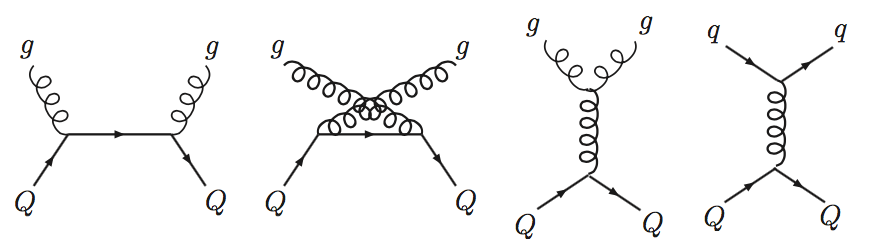
\includegraphics[width=14cm]{FigCap2/LO_HQscattering.png}
  \caption{Feynman diagrams for leading-order perturbative HQ scattering off light partons.}
  \label{fig:LoopCollScatt}
\end{figure}

The multiple scatterings of the heavy quark with the medium 
partons can also be treated as Brownian motion and typically
be described by the Boltzmann equation. In the limit of small 
momentum transfer, the latter can be reduced to the 
Fokker-Planck equation, which is often further reduced into the
Langevin equation. These
partial-differential equations can be used as transport equations, 
to describe the evolution of the momentum distribution
of heavy quarks along time. The Langevin equation for heavy-quark 
collisional energy loss presents itself as~\cite{Cao:2013ita}:
\begin{equation}
\label{eq:Langevin}
\frac{{\rm d} {\vec{p}}}{{\rm d} t} = - \eta_D (p) \vec{p} + \vec{\xi}.
\end{equation}
In Eq.~\ref{eq:Langevin}, the first right-hand side term is the 
deterministic friction force, while the second one ($ \vec{\xi}$) is the thermal random noise,
satisfying the properties:
\begin{equation}
\label{eq:Langevin2}
\langle {\xi^i (\pt)} {\xi^j (p_{\rm T'})} \rangle = b^{ij} (\pt) \frac{\delta_{tt'}}{{\rm d} t}, \; \; \; \; b^{ij} (\pt) = k_{\parallel}(p)\hat{p}^i\hat{p}^j + k_{\perp} (\delta^{ij} - \hat{p}^i\hat{p}^j).
\end{equation}
In Eq.~\ref{eq:Langevin2}, $k$ represents the momentum-space 
diffusion coefficient of heavy quarks;
the coefficient $\eta_D$ of Eq.~\ref{eq:Langevin2} is involved in the definition of the spatial 
diffusion coefficient $D_s$, which is related to the momentum-space 
diffusion coefficient via: 
\begin{equation}
\label{eq:Langevin3}
D_s = \frac{T}{M \eta_D} = \frac{2 T^2}{k}.
\end{equation}
To simulate the evolution of heavy quarks, one needs to discretise terms and calculate the increment 
$\vec{p}(t + \Delta t) -  \vec{p}(t)$ at a given time $t$. 

\subsection{Gluon-radiation processes}
\label{sec:rad}
While a parton is traversing the medium, it picks up some transverse 
momentum $k_{\perp}$ due to multiple scatterings. 
If we consider a gluon in the hard parton wave function, when the 
accumulated $k_{\perp}$ is enough, it can decohere from the partonic projectile and be emitted.
These are $1 \rightarrow 2$ processes, like $Q \rightarrow g\, Q$, 
where $Q$ is the heavy quark and $g$ the gluon.
The average phase $\phi$ of the gluon emitted with frequency $\omega$ on a distance $\Delta z$ is approximately:
\begin{equation}
\label{eq:gluonPhase}
\phi = {\Big \langle} \frac{k_{\perp}^2}{2\omega} \Delta z {\Big \rangle} \sim \frac{\hat{q} L}{2 \omega} L = \frac{\omega_c}{\omega},
\end{equation}
where $\hat{q}$ is the transport coefficient of the medium, 
defined as the average squared transverse 
momentum transferred to the projectile per average unit path 
length $L$: $\hat{q} = \langle k_{\perp}^2 \rangle / L$~\cite{Salgado:2003gb}.
Hence, gluons are emitted from the parton traversing a finite path 
length $L$ with a characteristic gluon frequency $\omega_c$:
\begin{equation}
\label{eq:gluonPhase}
\omega_c = \frac{1}{2} \hat{q} L^2.
\end{equation}
The distribution of energy $\omega$ of the radiated gluons, 
for small energies $\omega < \omega_c$ is of the form:
\begin{equation}
\label{eq:gluonEnDistrb}
\omega \frac{{\rm d} I}{{\rm d} \omega} \sim \frac{2 \alpha_s C_R}{\pi} \sqrt{ \frac{\omega_c}{2 \omega}},
\end{equation}
where $C_R$ is the Casimir factor for the QCD coupling, 
equal to 4/3 for quark-gluon coupling and to 3 for gluon-gluon coupling.
The $\omega$-integrated average parton energy loss results then (BDMPS formalism~\cite{Salgado:2003gb}):
\begin{equation}
\label{eq:RadEnLoss}
\langle \Delta E \rangle \propto \alpha_s \, C_R \, \hat{q} \, L^2. 
\end{equation}
We can then summarise the main properties of average parton 
energy loss via radiative processes:
\begin{itemize}
\item it grows with the path length like: $\Delta E \propto L^2$;
\item it is proportional to $\alpha_s C_R$, thus it is larger by a factor 
9/4 $ = 2.25$ for a gluon traversing the medium than for a quark;
\item it is independent of the initial parton energy $E$.
\end{itemize}
Furthermore, while in the limit of massless partons the probability of 
gluon emission is maximum for collinear radiation,
in the massive limit the soft-gluon emission probability, for small 
emission angles $\Theta \ll 1$, is~\cite{Dokshitzer:1991fd}:
\begin{equation}
\label{eq:DeadCone}
{\rm d} \sigma_{Q \rightarrow gQ } \sim \frac{\Theta^2 {\rm d} \Theta^2}{[\Theta^2+ \Theta^2_0]} \frac{{\rm d} \omega}{\omega},
\end{equation}
with $\Theta_0 = M_Q/E_Q$.
Therefore, in the kinematical region $\Theta < \Theta_0$ the yield of radiated gluons
in the forward direction provides a small contribution to the total multiplicity of emitted gluons. 
The depleted forward region is called the {\it dead cone}~\cite{Dokshitzer:1991fd}.
Since $\Theta_0 = M_Q/E_Q$, the effect is expected to be more 
relevant with increasing parton mass. A hierarchy in 
the energy loss is hence expected:
\begin{equation}
\label{eq:HierachyRaa}
\Delta E_{gluon} > \Delta E_{light\, quark} > \Delta E_{heavy\, quark},
\end{equation}
where the first inequality comes from the different couplings in $gg$ and $gq$ 
processes due to the Casimir factor in Eq.~\ref{eq:gluonEnDistrb} 
and the second from the dead-cone effect. The hierarchy, if present, 
should consequently affect the $\RAA$ values of hadrons originating from
gluon, light and heavy-quark fragmentation.\\


\begin{figure}[!ht]
  \centering
  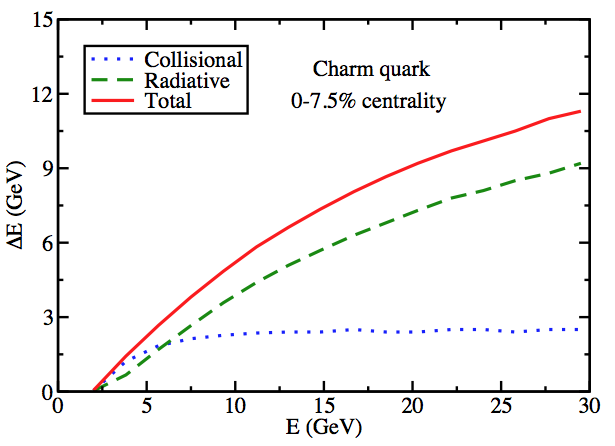
\includegraphics[width=7cm]{FigCap2/HFEnLoss1.png}
  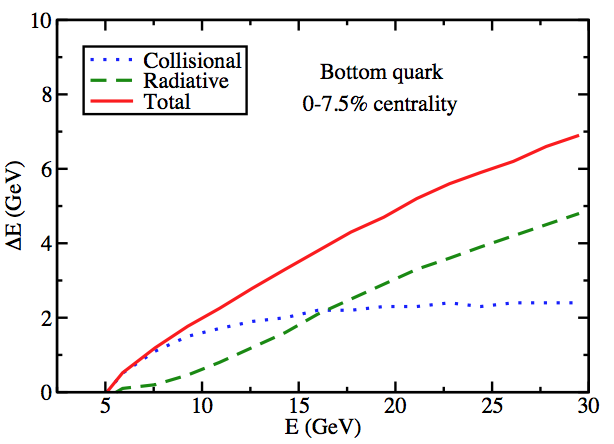
\includegraphics[width=7cm]{FigCap2/HFEnLoss2.png}
  \caption{Comparison of radiative and collisional energy losses for charm (left) and for bottom (right) quarks as a function of the quark energy from calculations in~\cite{Cao:2013ita}.}
  \label{fig:HFEnLoss}
\end{figure}
In Fig.~\ref{fig:HFEnLoss}, an example of calculations from~\cite{Cao:2013ita}
for the energy loss of charm (left) and beauty (right) quarks 
in central Pb-Pb collisions at the LHC is shown as a function of the initial energy of the quark.
In the model~\cite{Cao:2013ita}, quarks evolve in a static medium at a temperature
$T = 300$ MeV according to a Langevin equation (like that in Eq.~\ref{eq:Langevin}) with 
an additional term for radiative contribution. 
Both the contributions from collisional and radiative energy loss 
are displayed in Fig.~\ref{fig:HFEnLoss}. Elastic interactions
dominate the low-$\pt$ region, up to $\sim 6\; \Gevc$ for charm and $\sim 16 \;\Gevc$ for beauty quarks.
At higher $\pt$, the contribution from radiative processes is the dominant one and must be considered when 
performing calculations at LHC energies.
It is also interesting to look at Fig.~\ref{fig:HFEnLoss2} (left), always from the
same calculations~\cite{Cao:2013ita}, that shows the 
thermalisation process of charm quarks in the medium as a function of time.
The initial energy of the charm quarks is 10 GeV. Depending on the different implementation for energy
loss, the thermalisation of the charm quarks occurs at different times.\\
\begin{figure}[!ht]
  \centering
  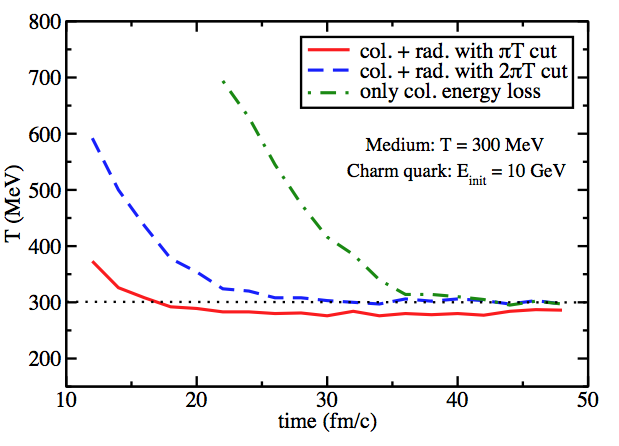
\includegraphics[width=7cm]{FigCap2/HFEnLoss3.png}
  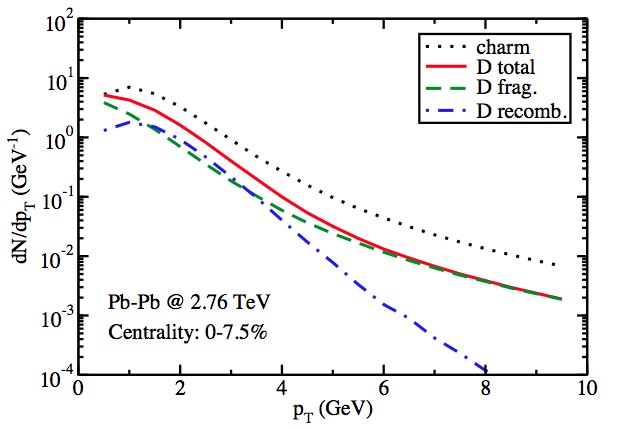
\includegraphics[width=7cm]{FigCap2/FragHQ.png}
  \caption{Left: thermalisation process of charm quarks in a static medium~\cite{Cao:2013ita}. Right: relative contributions from different hadronisation mechanisms to D-meson production  from charm quarks, as a function of the transverse momentum, from calculations in~\cite{Cao:2013ita}.}
  \label{fig:HFEnLoss2}
\end{figure}

\subsection{Heavy flavour hadronisation in the medium}
\label{sec:HFhadro}

The final hadron yields and momentum distributions not only depend on the energy loss 
mechanisms of the partons inside the medium,
but also on the way parton hadronisation occurs. There are basically 
two mechanisms for heavy quarks 
to produce heavy-flavour hadrons: fragmentation of a 
heavy quark into a jet of lower-momentum
hadrons, or coalescence (re-combination) of low-momentum 
quarks with partons from the 
medium. Figure~\ref{fig:HFEnLoss2} (right) illustrates the 
contributions of coalescence and fragmentation 
mechanisms into the final D-meson yields from charm-quark 
hadronisation in central Pb-Pb collisions at the LHC. The recombination mechanism
gives an important contribution at low $\pt$, while the independent 
fragmentation dominates at higher $\pt$.
Since the coalescence with partons from the medium gives rise to a 
hadron with momentum larger than that of the 
heavy quark, the $\pt$ distribution of the final hadrons produced via coalescence will be slightly 
harder than that of the initial quarks,
i.e. shifted towards higher momenta. A remarkable example
for the study of heavy-quark hadronisation processes and the role of coalescence is the production of J/$\psi$ meson,
discussed in Sec.~\ref{sec:Quarkonium}.\\



The measurement of $\Ds$-meson production in A-A collisions can provide 
crucial additional information to understand the 
interactions of charm quarks with the strongly-interacting 
medium formed in heavy-ion collisions at high energies.
In particular, the $\Ds$-meson yield is sensitive to strangeness production 
and to the hadronisation mechanism of charm quarks.
The enhancement of strange particle production in presence of QGP was already discussed in
Sec.~\ref{subsec:StrangEnhancSPS} and a pattern of strangeness 
enhancement increasing with the hadron strangeness 
content when going from pp to p-A and then to heavy-ion collisions was observed at 
the SPS~\cite{NA57_158,NA57_40,NA49_Kpi,NA49_LambdaXi}, at
RHIC~\cite{STAR_hyperons} and at the LHC~\cite{ALICE:2017jyt}.
This strangeness enhancement effect could also affect the production of 
charmed hadrons if the dominant mechanism for D-meson formation at 
low and intermediate momenta is in-medium hadronisation of charm quarks via 
recombination with light quarks.
Under these conditions, the relative yield 
of $\Ds$ mesons with respect to non-strange charmed mesons at low $\pt$ is predicted to be enhanced
in nucleus-nucleus collisions as compared to pp 
interactions~\cite{Andronic2003,RafelskiKuznetsova,HeFriesRapp}.
The comparison of the $\pt$-differential production yields 
of non-strange D mesons and of $\Ds$ mesons in A-A and pp 
collisions is therefore sensitive to the role of recombination in charm-quark 
hadronisation.
\begin{figure}[!h]
  \centering
  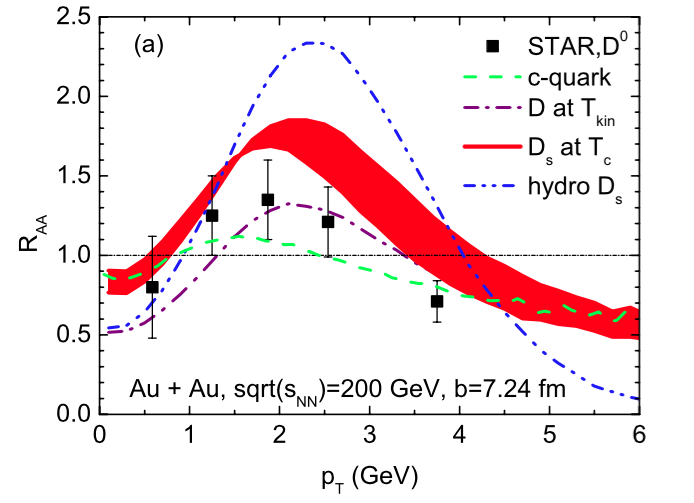
\includegraphics[width=7cm]{FigCap2/RaaDsRapp.png}
  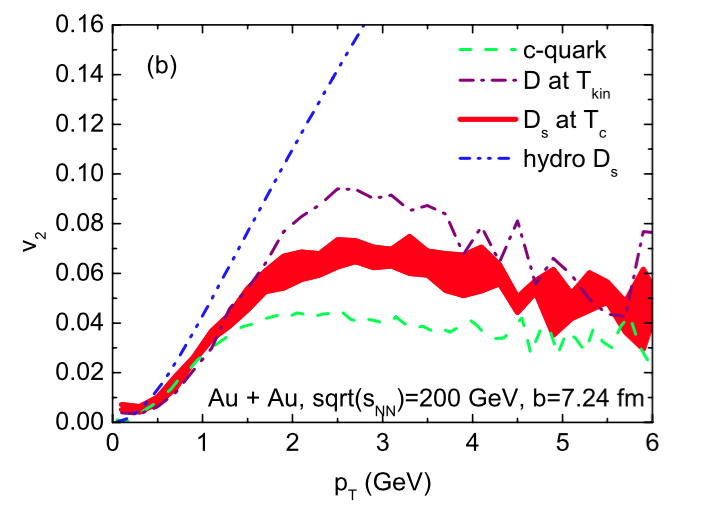
\includegraphics[width=7cm]{FigCap2/v2DsRapp.png}
  \caption{Results for the $\RAA$ (left panel) and $v_2$ (right) of $\Ds$ (red bands) and D (purple dashed-dotted lines) mesons in semi-central Au-Au collisions at RHIC~\cite{He:2012df}. Results for charm quarks at pseudo-critical temperature $T_c$ (green dashed lines), the equilibrium limit for $\Ds$ meson in the hydrodynamic medium at $T_{c}$ (blue dashed-double-dotted line) and STAR data for the $\Dzero$-meson $\RAA$ in in 0-80\% Au-Au collisions are also reported~\cite{Zhang:2011uva}.}
  \label{fig:Rapp}
\end{figure}
Figure~\ref{fig:Rapp} shows D- and $\Ds$-meson $\RAA$ (left-hand panel)
and $v_2$ (right), in semi-central Au-Au collisions at 
RHIC, from the TAMU model calculations~\cite{He:2012df}, also
compared to STAR measurements of $\Dzero$-meson $\RAA$ in 0-80\% Au-Au 
collisions~\cite{Zhang:2011uva}.
The model predicts the maximum $\RAA$ to be more 
pronounced for the $\Ds$, reaching values larger than 1.5 due 
to $c$-quark coalescence with the enhanced strangeness in Au-Au.
In the calculations of the model, the elliptic flow coefficient results to be sensitive both 
to the collectivity of the medium and to hadronization. Thanks to the coalescence of charm quarks with 
thermal light and strange quarks, the flow coefficients of non-strange D and $\Ds$ mesons reach
values larger by $\sim$50\% than the $v_2$ of charm quarks. Furthermore, interactions of non-strange D mesons
with the medium constituents during the hadronic phase create a further 30\%
difference between strange and non-strange D-meson $v_2$.

\iffalse
A consequence of the possibly enhanced production of $\Ds$ mesons in heavy-ion 
collisions would be a slight reduction of the fraction of charm quarks 
hadronising into non-strange meson species.
Therefore, the measurement of the $\Ds$-meson production is also relevant
for the interpretation of the comparison of the nuclear modification
factors of non-strange D mesons and light-flavour 
hadrons (pions)~\cite{ALICEDRAA,Adam:2015sza}, which is predicted 
to be sensitive to the quark-mass and colour-charge dependence of parton 
in-medium energy loss~\cite{ADSW,WHDG,Djordjevic}.
Furthermore, due to this possible modification of the relative abundances
of D-meson species, measuring the $\Ds$ yield at low $\pt$ is needed 
also to determine the total charm production cross section in Pb--Pb 
collisions.
\fi

\begin{figure}[!ht]
  \centering
    \includegraphics[width=7cm]{FigCap2/AverageDmesonRaa_010_DzeroSTAR_010.pdf}
    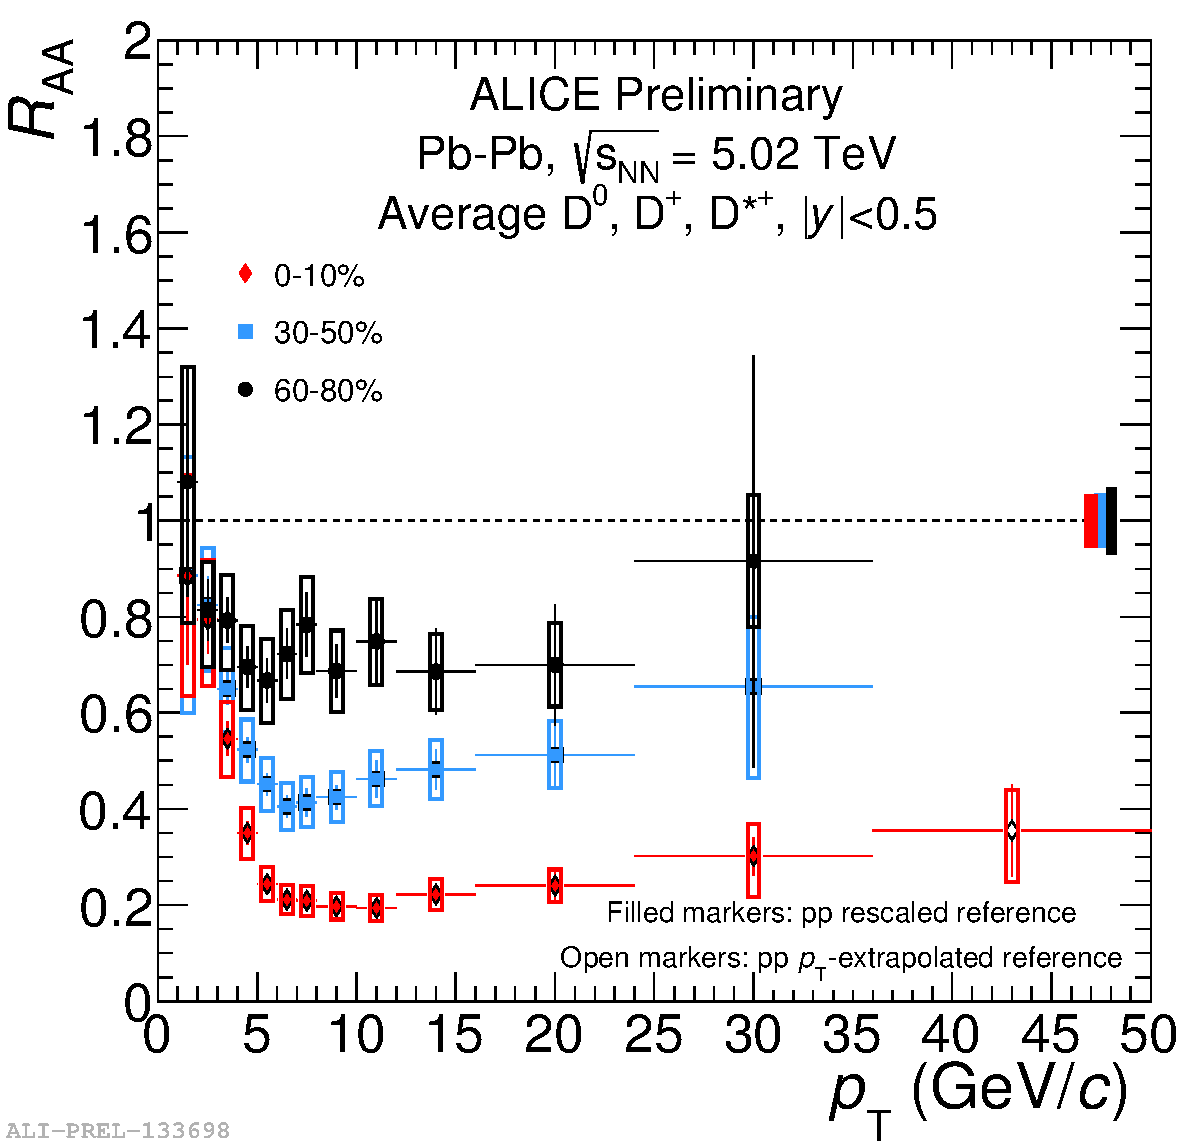
\includegraphics[width=7cm]{FigCap2/2017-Jul-05-DmesonAverage_010_3050_6080_comparison_04July2017.pdf}
  \caption{Left: average non-strange D-meson $\Raa$ as a function of $\pt$ in the 10\% most central Pb-Pb collisions at
 $\sNN=2.76$ TeV measured by ALICE~\cite{Adam:2015sza}, compared to $\Dzero$ $\Raa$ measured by the STAR Collaboration in 0-10\% Au-Au collisions at RHIC at
$\sNN=200$ GeV~\cite{Adamczyk:2014uip}. A zoomed-in plot of the interval $0 < \pt < 8\, \Gevc$ is shown in the inset. Right: average $\RAA$ 
  of prompt $\Dzero$, $\Dplus$ and $\Dstar$ mesons in the 0--10\% (red), 30--50\% (blue) and 60--80\% (black) centrality classes at $\sqrtsNN=5.02~\tev$~\cite{ALICE-PUBLIC-2017-003}.  }
  \label{fig:Raa}
\end{figure}

\subsection{Experimental results in A-A collisions}
\label{sec:resAAcap2}
In the left-hand panel of Fig.~\ref{fig:Raa}, the average D-meson $\RAA$ 
for the 10\% most central Pb-Pb collisions at $\sNN = 2.76$ TeV 
measured by ALICE~\cite{Adam:2015sza} is compared to the $\Dzero$ 
nuclear modification factor measured by the STAR Collaboration
for the 10\% most central Au-Au collisions at $\sNN = 200$ GeV~\cite{Adamczyk:2014uip}. 
The nuclear modification factors measured at the two energies are compatible within uncertainties for $\pt > 2\, \Gevc$.
Similar $\RAA$ of D mesons for $\pt > 5 \,\Gevc$ does not necessarily imply a similar charm-quark
energy loss at the two collision energies. A combined effect of a denser medium
and of the harder $\pt$ spectra at the LHC could result in similar values of $\RAA$ at lower
collision energies~\cite{Baier:2002tc}. In the interval $1 < \pt < 2\, \Gevc$, the $\RAA$ 
measured by STAR shows a maximum. This effect can be described 
by models including parton energy loss, collective
radial flow and the contribution of the recombination mechanism to 
charm-quark hadronisation~\cite{Abelev:2006db}. The ALICE results at higher energy 
do not show a maximum. Several effects can explain differences at the two energies, 
due to the different role of initial-state effects or of radial flow at the 
two collision energies. In the initial state, the modification
of the parton distribution functions in a nuclear environment is predicted to lead
to a stronger suppression of the heavy-quark production yields at low $\pt$ with increasing
$\sNN$~\cite{Eskola:2009uj}, because of the smaller values of Bjorken-x probed 
and therefore more shadowing is expected. In addition, the 
$k_{\rm T}$-broadening effect, which gives rise to an enhancement of the $\RAA$ at low-intermediate
$\pt$ (Cronin peak), is known to be more pronounced at lower collision energies~\cite{Wang:1998ww,Vogt:2001nh}.
In the final state, in addition to energy loss, the collective expansion of the medium is
also predicted to affect the momentum distribution of charmed hadrons in heavy-ion collisions.
This effect could be enhanced by hadronisation via recombination.
The stronger radial flow (see Sec.~\ref{sec:RadialFlow}) at the LHC than at 
RHIC~\cite{Abelev:2008ab,Abelev:2013vea,Abelev:2012wca} does not necessarily give rise
to a more pronounced bump-like structure in the $\RAA$ at low $\pt$ with increasing collision
energy. Its effect can in fact be counterbalanced by the different shape of the momentum
spectra in pp collisions at different energies. Reduced uncertainties
on the measurements are needed to draw firmer conclusions.\\
Preliminaries results of the average nuclear modification factors 
of $\Dzero$, $\Dplus$ and $\Dstar$ as a function of
$\pt$ measured in Pb-Pb collisions at $\sNN = 5.02 $ TeV 
are shown in Fig.~\ref{fig:Raa} (left), 
for the 0--10\%, 30--50\% and 60--80\% centrality classes~\cite{ALICE-PUBLIC-2017-003}. 
The D-meson nuclear modification factors at $\sNN = 5.02$ TeV 
exhibit a suppression which is compatible within uncertainties 
with that measured at lower energy $\sNN = 2.76$ TeV~\cite{Adam:2015sza}. 
The suppression is maximal at $\pt=6$--$10~\gev/c$ for central and semi-central events, 
where a reduction of the yields by
a factor of about 5 and 2.5 with respect to the binary-scaled pp reference is observed 
in the two centrality classes, respectively.
The suppression decreases with decreasing $\pt$ for $\pt<6~\GeV/c$, and 
$\RAA$ is compatible with unity  in the interval $1<\pt<3~\gev/c$.
The average $\RAA$ in the 60--80\% centrality class shows a suppression 
by about 20--30\%, without a pronounced dependence on $\pt$. 
Recent studies proposed that event selections and geometry determination 
of the collision can bias the $\RAA$, causing
an artificial suppression for $\RAA$ in peripheral collisions even in absence
of jet quenching and shadowing~\cite{Morsch:2017brb}.\\


The $\RAA$ of prompt $\Ds$ mesons in the 10\% most central Pb-Pb collisions 
at $\sNN =  2.76$ TeV is compared in the left-hand panel
of Fig.~\ref{fig:DsD_MassDep} to the average nuclear modification factor of 
$\Dzero$, $\Dplus$ and $\Dstar$ mesons measured in the same
centrality class~\cite{Adam:2015sza}. This comparison is meant to 
address the expected effect of hadronisation via quark
recombination in the partonic medium on the relative abundances 
of strange and non-strange D-meson
species. In the three $\pt$ intervals, the values of the $\Ds$-meson $\RAA$ 
are higher than those of non-strange D mesons, although 
compatible within the large uncertainties. More precise measurements are 
expected with the data sample from LHC Run 2 at $\sNN = 5.02$ TeV and are the subject of this thesis.\\
\begin{figure}[!ht]
  \centering
    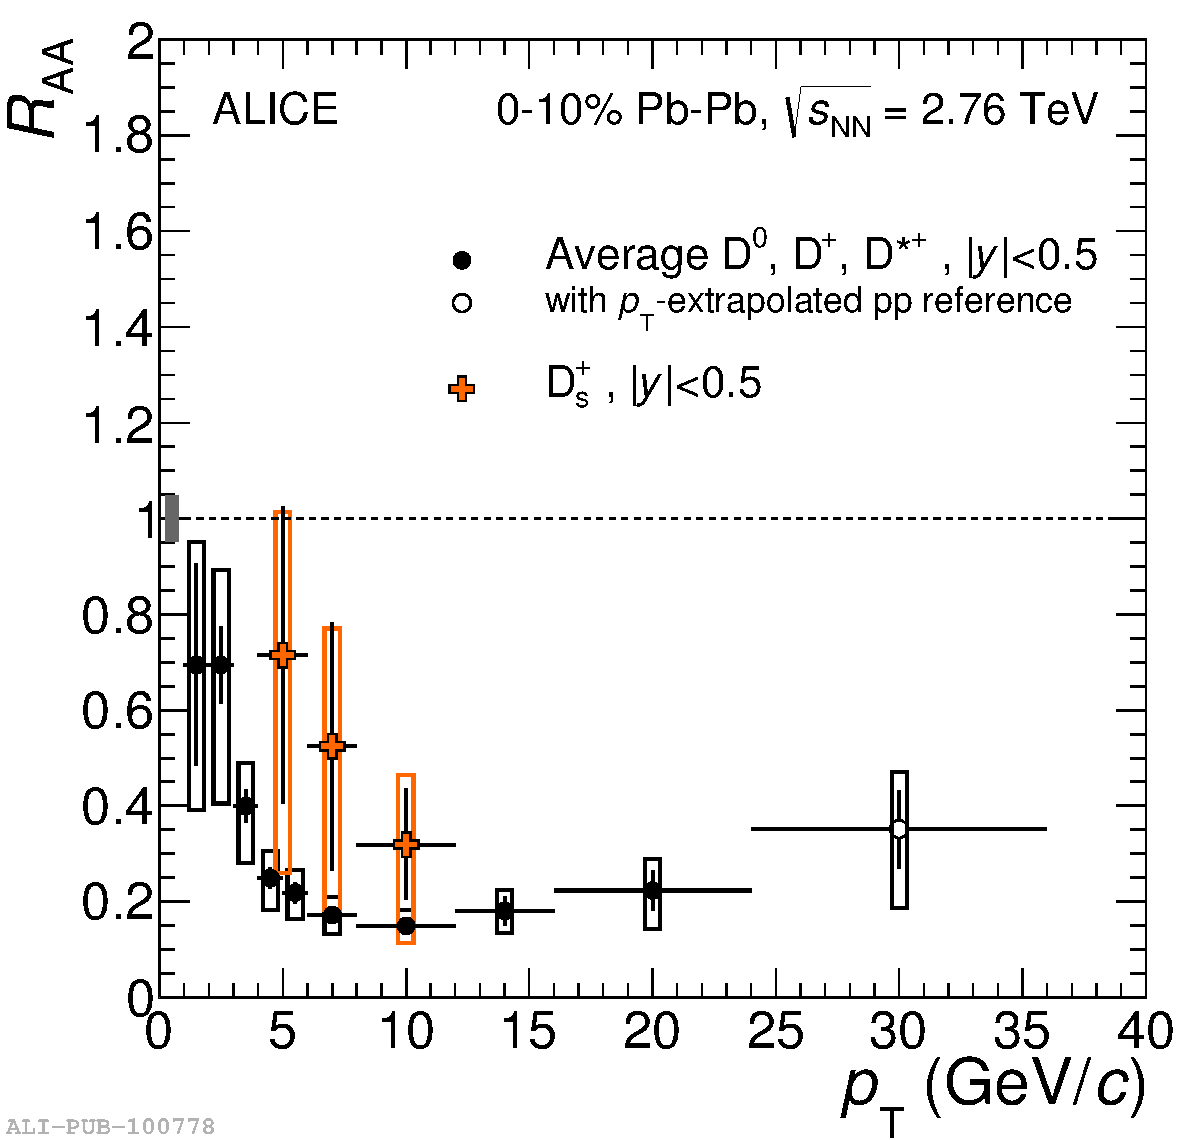
\includegraphics[width=7.1cm]{FigCap2/RAADsD_276.pdf}
    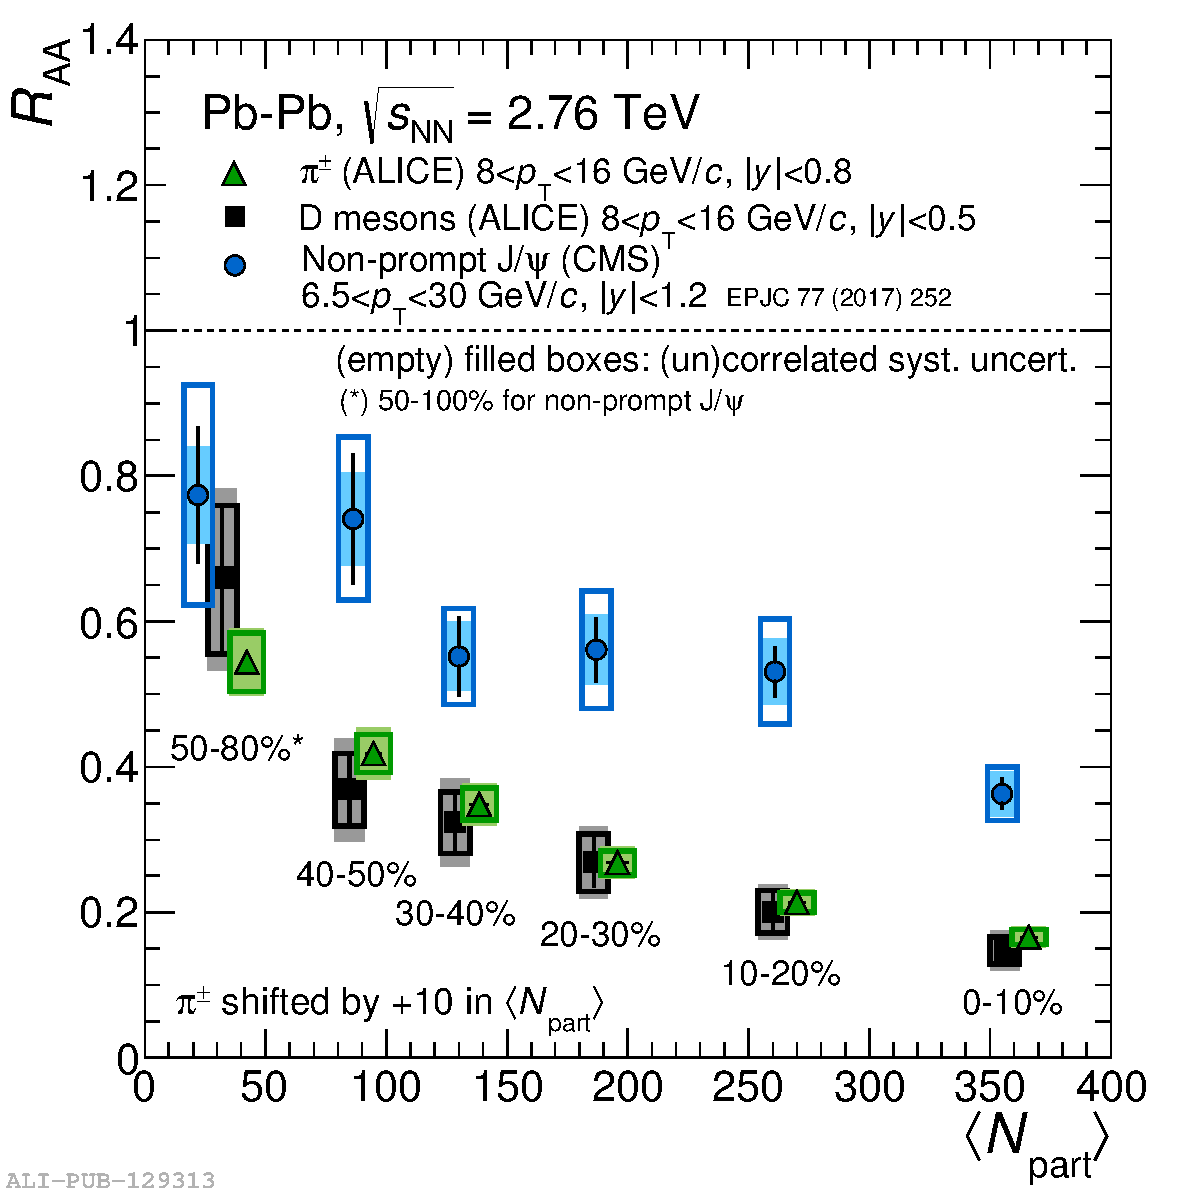
\includegraphics[width=6.9cm]{FigCap2/2017-May-22-RaavsNpart_Dmes8to16_Pions8to16_FinalNonPromptJpsi2017_CC_25042017.pdf}
  \caption{Left: $\RAA$ of prompt $\Ds$ mesons~\cite{Adam:2015jda} compared to non-strange D mesons~\cite{Adam:2015sza} in the 0-10\% centrality class at $\sNN = 2.76$ TeV. Right: Comparison of the D-meson~\cite{Adam:2015nna} and charged-pion~\cite{Abelev:2014laa} $\RAA$ as a function of centrality expressed in terms of $\langle N_{\rm part} \rangle $ in \mbox{8 $< \pt < 16$ $\Gevc$} measured by ALICE~\cite{Adam:2015nna}, 
and of the $\RAA$ of non-prompt J$/\psi$ mesons in 6.5 $< \pt < 30$ $\Gevc$ measured by CMS~\cite{Khachatryan:2016ypw}. 
}
  \label{fig:DsD_MassDep}
\end{figure}

\begin{figure}[!ht]
  \centering
    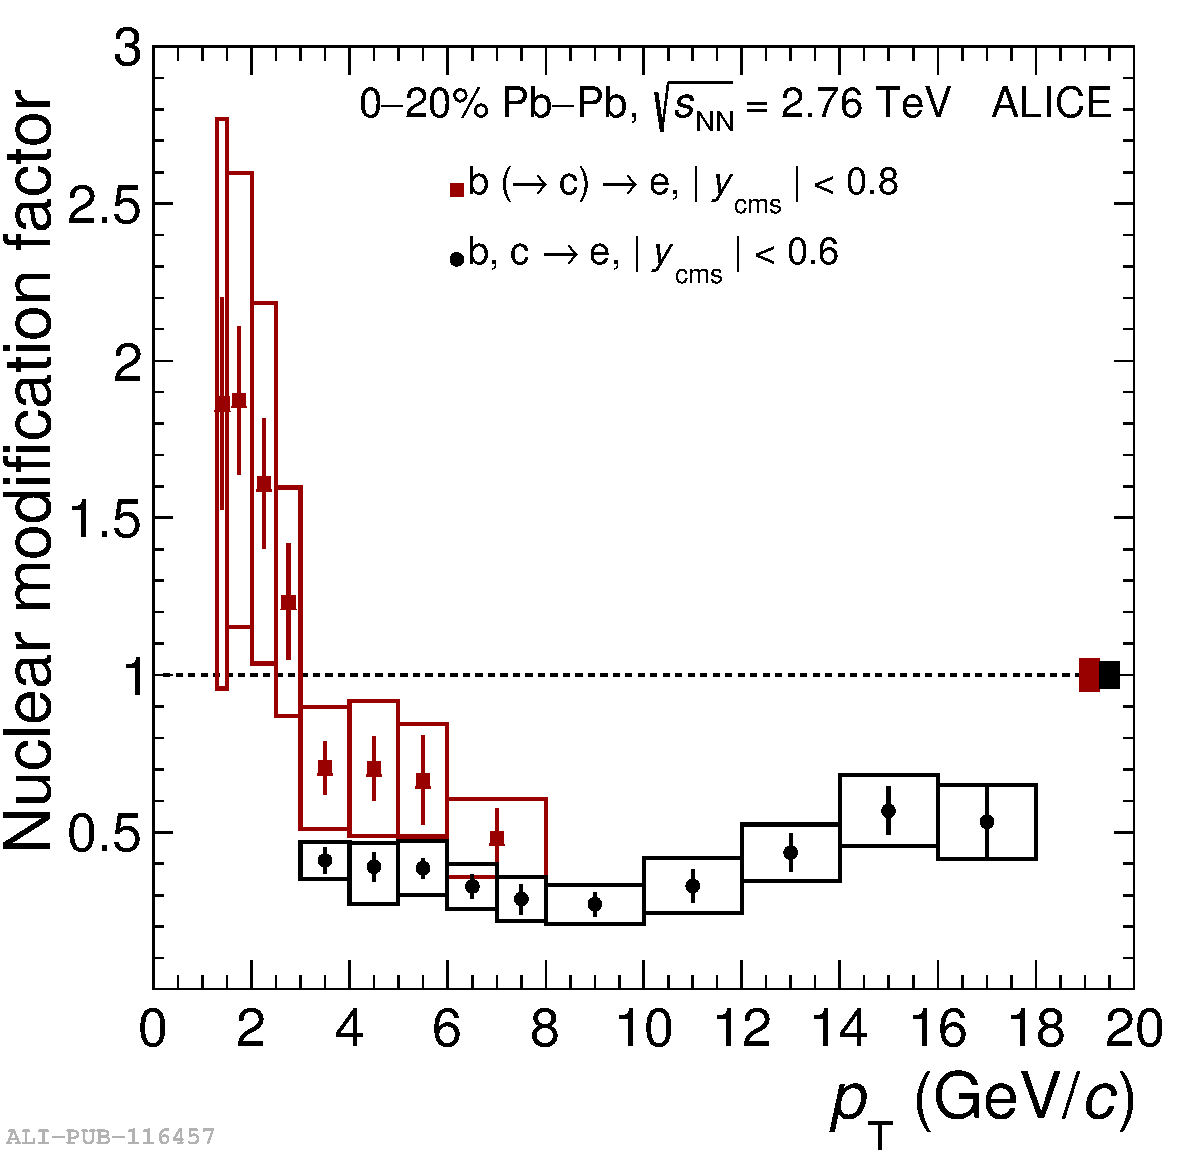
\includegraphics[width=7.5cm]{FigCap2/2017-Jan-28-rParAAbeautyincl.pdf}
  \caption{Right: $\RAA$ of electrons from beauty-hadron decays as a function of $\pt$ together with
the corresponding result for beauty- and charm-hadron decays~\cite{Adam:2016khe} for the 20\% most central Pb-Pb collisions at $\sNN=2.76$ TeV.}
  \label{fig:ColorMassDep}
\end{figure}

Figure~\ref{fig:DsD_MassDep} (right) shows the average of the $\Dzero$, $\Dplus$ and $\Dstar$ 
nuclear modification factors as a function of centrality measured by ALICE in
Pb-Pb collisions at $\sNN =  2.76$ TeV, for the interval 8 $< \pt < 16$ $\Gevc$  in $|y| < 0.5$~\cite{Adam:2015nna}, 
compared to the $\RAA$ of charged pions~\cite{Abelev:2014laa} in $|y| < 0.8$ for the same $\pt$ interval, 
and to non-prompt J$/\psi$ meson $\RAA$ measured by the CMS Collaboration for 6.5 $< \pt < 30$ $\Gevc$ 
in $|y| < 1.2$~\cite{Khachatryan:2016ypw}. The different width of the rapidity interval for D and non-prompt
J$/\psi$ mesons ($|y| < 0.5$ and $|y| < 1.2$, respectively) is not expected to play a big role, since
the intervals are partially overlapping and there is no significant $y$ dependence of the $\RAA$ of 
non-prompt J$/\psi$ mesons in $|y| < 1.2$~\cite{Khachatryan:2016ypw}. 
The $\pt$ interval 8-16 $\Gevc$ for D mesons was chosen 
in order to obtain a significant overlap with the $\pt$ distribution 
of B mesons decaying to J/$\psi$ particles with $6.5 < \pt < 30\, \Gevc$.
The nuclear modification 
factors of charged pions and D mesons are compatible within uncertainties
in all centrality classes. A possible interpretation of the similar $\RAA$ of D mesons and pions is 
related to a mixture of competitive effects which affect the nuclear modification
factor in addition to the parton in-medium energy loss. In particular,
in the presence of a colour-charge and quark-mass dependent 
energy loss, the harder $\pt$ distribution and the harder fragmentation function of 
charm quarks compared to those of light quarks and gluons could lead to similar 
values of D-meson and pion $\RAA$, as discussed in~\cite{Djordjevic:2013pba}. 
The value of the D-meson $\RAA$ in all the centrality
classes, except the most peripheral one, is lower than that of non-prompt J$/\psi$ mesons. 
The $\RAA$ of electrons from beauty-hadron decays~\cite{Adam:2016wyz} 
is compared with the one of heavy-flavour decay electrons, i.e. originating from both charm- and
beauty-hadron decays, in Fig.~\ref{fig:ColorMassDep} 
for the 20\% most central Pb-Pb collisions
~\cite{Adam:2016khe}. The measurements agree within 
uncertainties at high $\pt$, while, in the $\pt$ 
interval 3 $< \pt < 6$ $\Gevc$, the $\RAA$ 
of electrons from beauty-hadron decays 
is about 1.2$\sigma$ higher than that of heavy-flavour decay 
electrons. The observation of different 
suppression for particles originating from
charm or beauty quarks like those presented in Fig.~\ref{fig:DsD_MassDep} (right) and~\ref{fig:ColorMassDep} 
is consistent with a scenario of decreasing in-medium 
parton energy loss with increasing quark mass.\\

\begin{figure}[!ht]
  \centering
        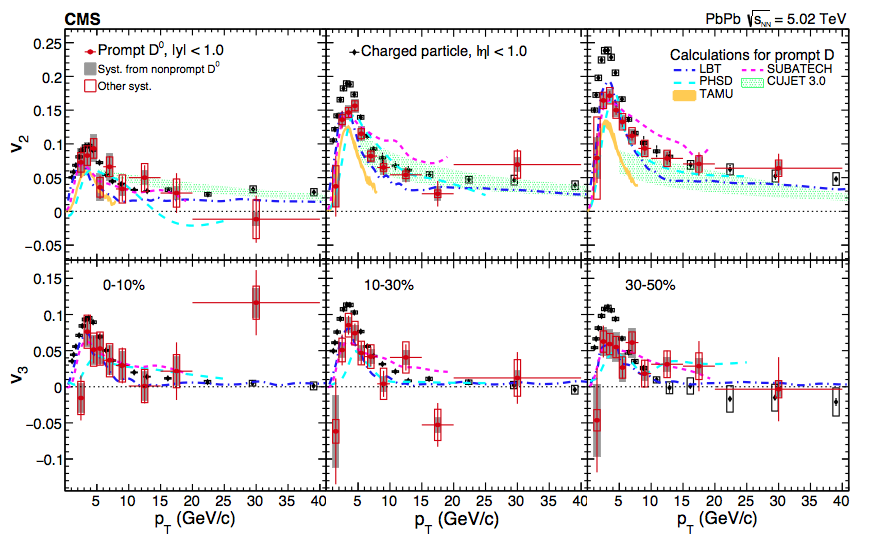
\includegraphics[width=14cm]{FigCap2/D0v2_CMS_5TeV.png}
  \caption{Prompt $\Dzero$ meson $v_2$ (upper) and $v_3$ (lower) coefficients as a function of $\pt$ at midrapidity ($|y| < 1.0$) for
the centrality classes 0-10\% (left), 10-30\% (middle), and 30-50\% (right)~\cite{Sirunyan:2017plt}.}
  \label{fig:D0v2CMS}
\end{figure}



The measurement of the elliptic flow $v_2$ provides further 
insight into the interactions of charm quarks with the medium. 
At low $\pt$, D-meson $v_2$ offers the unique opportunity 
to test whether also charm quarks participate in the collective 
expansion dynamics and possibly thermalize in the medium~\cite{Greco:2003vf,Ollitrault:1992bk}. 
At low and intermediate $\pt$, the elliptic flow is also expected to 
be sensitive to the hadronization mechanism~\cite{Greco:2003vf}, while at high $\pt$, 
it can constrain the path-length dependence of parton energy loss~\cite{Gyulassy:2000gk}.
First measurements of a positive D-meson $v_2$ were done by ALICE
in Pb-Pb collisions at $\sNN = 2.76$ TeV~\cite{Abelev:2014ipa}.
The $v_2$ and $v_3$ of prompt $\Dzero$ meson measured by CMS 
in Pb-Pb collisions at $\sNN = 5.02 $ TeV are presented in 
Fig.~	\ref{fig:D0v2CMS}, for the 0-10\%, 
10-30\% and 30-50\% centrality classes ~\cite{Sirunyan:2017plt}. 
The measured $v_2$ and $v_3$ are larger than 0 
at low $\pt$ and then decrease at higher $\pt$.
The elliptic flow $v_2$ reaches its maximum value in the 30-50\% centrality class,
due to the initial geometrical anisotropy of the fireball.
The result suggests that charm quarks take part in 
the collective motion of the medium and that collisional processes as well as quark 
recombination may contribute to the observed elliptic flow. 
For $\pt > 6\, \Gevc$, the $\Dzero$ meson $v_2 >0$ suggests a 
path-length dependence of the charm-quark energy loss. 
The path-length effect is more evident for semi-peripheral collisions, where the difference of
in-plane and out-of-plane path-lengths is maximum.\\


\begin{figure}[!ht]
  \centering
    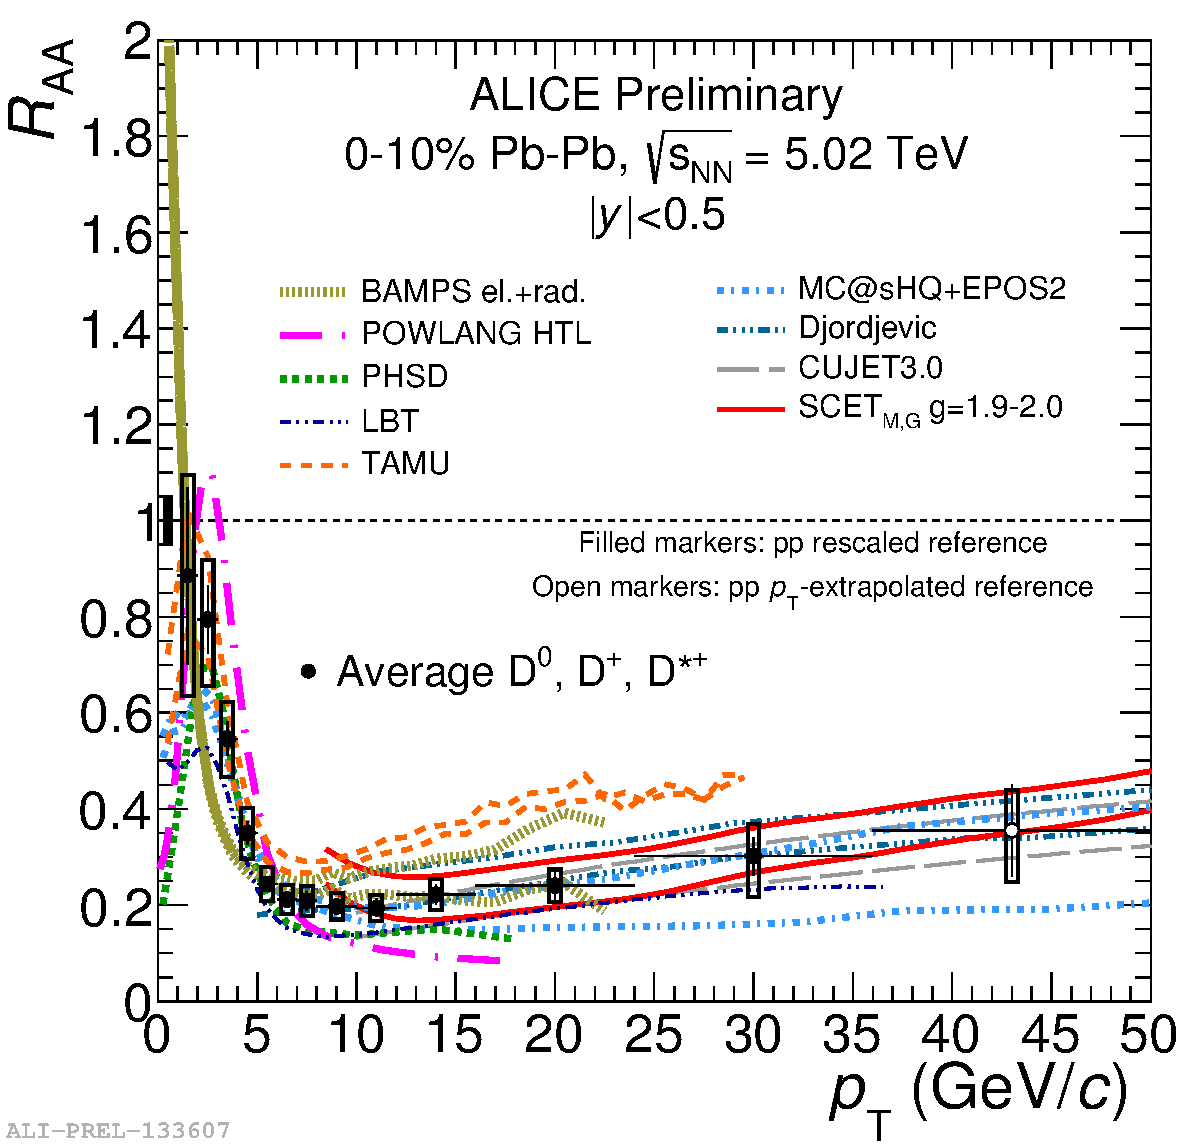
\includegraphics[width=7cm]{FigCap2/2017-Jul-07-DmesonAverage_010_All_Models_04July2017.pdf}
    \includegraphics[width=7cm]{FigCap2/DmesonAverage_3050_AllModels_18May2017.pdf}
    \includegraphics[width=7cm]{FigCap2/DmesonAverage_6080_All_Mod04July2017.pdf}
  \caption{Average D-meson $\RAA$~\cite{ALICE-PUBLIC-2017-003} in 0-10\%, 30-50\% and 60-80\% centrality classes as a function of $\pt$ at $\sNN = 5.02$ TeV, compared with models.}
  \label{fig:RAADs}
\end{figure}



\begin{figure}[!ht]
  \centering
    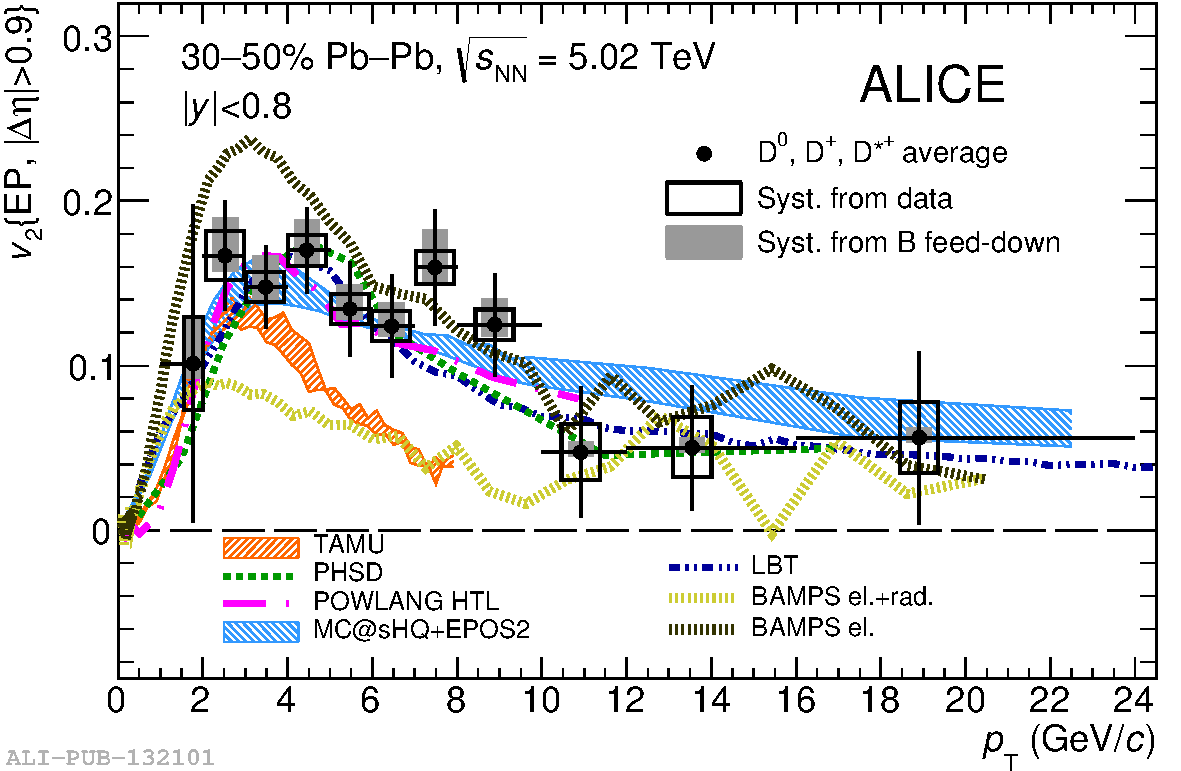
\includegraphics[width=11cm]{FigCap2/2017-Jul-04-DmesonComparisonWithModels.pdf}
%    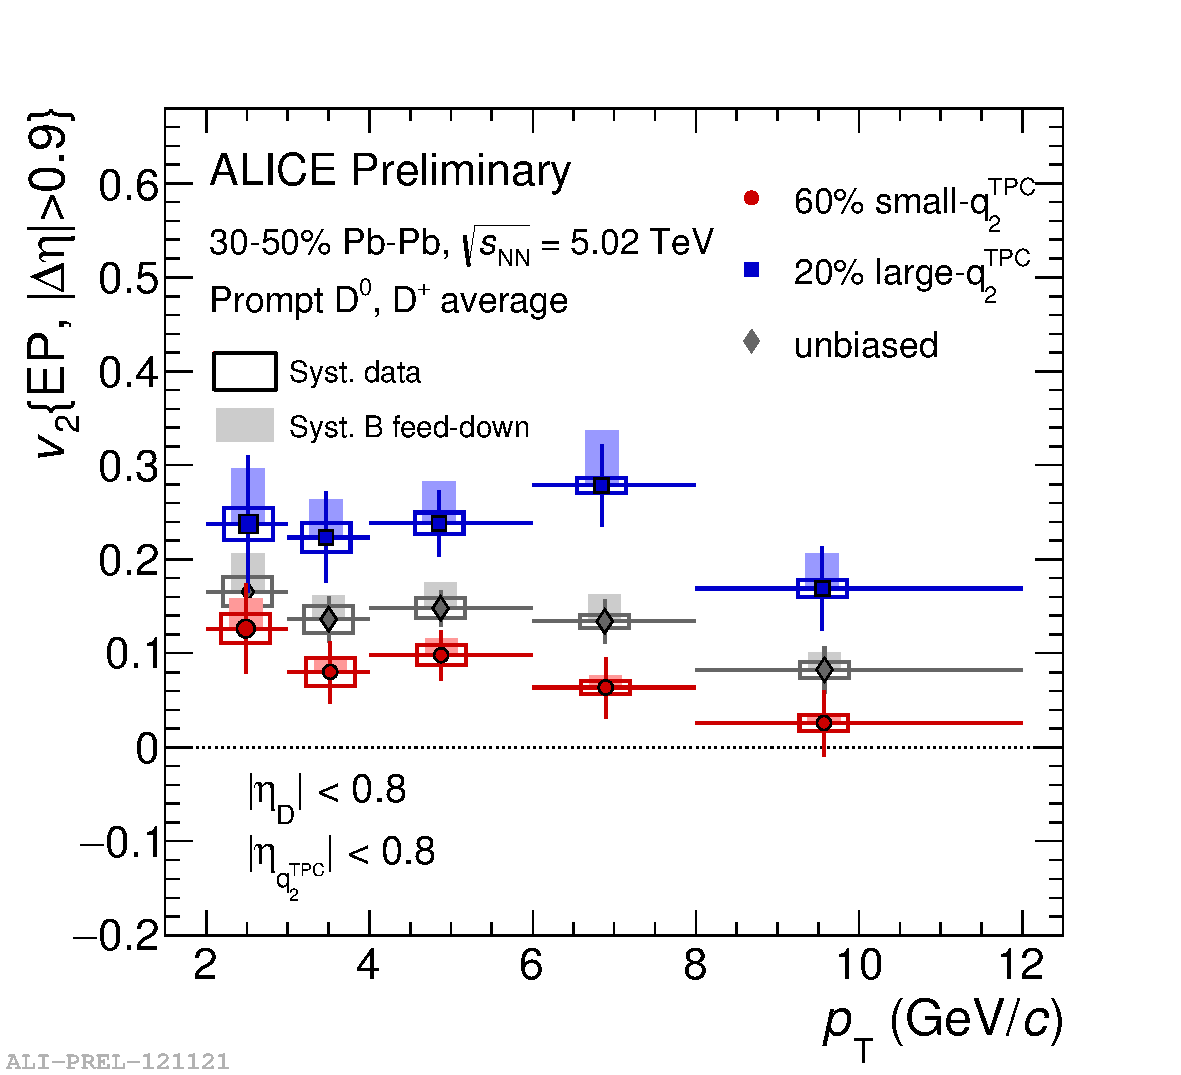
\includegraphics[width=7cm]{FigCap2/2017-Sep-13-v2ESE_Daverage_PbPb3050_VZERO_q2TPCFullSmall60Perc_q2TPCFullLarge20perc.pdf}
  \caption{Average D-meson $v_2$~\cite{Acharya:2017qps} in the 30-50\% centrality class as a function of $\pt$ at $\sNN = 5.02$ TeV, compared with models.}
  \label{fig:Dmesonsv2}
\end{figure}

The simultaneous comparison of $\RAA$ and elliptic flow $v_2$ measurements 
with theoretical calculations can provide more stringent constraints to the 
charm-quark in-medium interactions and hadronisation processes.
Fig.~\ref{fig:RAADs} shows the D-meson $\RAA$~\cite{ALICE-PUBLIC-2017-003}  
measured by ALICE in Pb-Pb collisions at $\sNN = 5.02$ TeV, in the 0-10\%, 30-50\% and 60-80\% 
centrality classes and Fig.~\ref{fig:Dmesonsv2} shows the D-meson $v_2$~\cite{Acharya:2017qps} in the 30-50\% 
centrality class.
Transport models in Fig.~\ref{fig:RAADs} and~\ref{fig:Dmesonsv2} include: 
POWLANG~\cite{Beraudo:2014boa} and TAMU~\cite{He:2014cla}, 
in which the interactions only include collisional processes; 
BAMPS-el+rad~\cite{Uphoff:2014hza}, LBT~\cite{Cao:2017hhk} and 
PHSD~\cite{Song:2015ykw}, in which also energy loss from medium-induced gluon radiation
is considered, in addition to collisional process.
Models based on perturbative QCD calculations of parton energy loss 
are: CUJET3.0~\cite{Xu:2015bbz}, Djordjevic~\cite{Djordjevic:2015hra} 
and MC@sHQ+EPOS2~\cite{Nahrgang:2013xaa}, that include both radiative 
and collisional energy loss processes, and SCET~\cite{Kang:2016ofv} model, that includes 
medium-induced gluon radiation and a mechanism of formation and dissociation of 
heavy-flavour hadrons in the QGP. All models, with the exception of BAMPS and CUJET3.0, 
include a nuclear modification of the parton distribution functions.
The LBT, MC@sHQ, PHSD, POWLANG and TAMU
models include a contribution of hadronisation via quark recombination, 
in addition to independent fragmentation. 
Most of the models provide a fair description of the measured $\RAA$ in the region 
$\pt<10~\gev/c$ in central collisions, 
but many of them (LBT, PHSD, POWLANG and SCET) provide a worse 
description of non-central collisions.
%In the high-$\pt$ region above $10~\gev/c$ only the BAMPS, CUJET3.0, 
%Djordjevic and SCET models can describe the data. 
The CUJET3.0 and Djordjevic models provide a fair description of the $\RAA$ in all three 
centrality classes for $\pt > 5-10~\gev/c$, where radiative energy loss 
is expected to be the dominant interaction mechanism, suggesting that 
the dependence of radiative energy loss on the path length of charm 
quarks in the hot and dense medium is well understood. 
The TAMU model overestimates $\RAA$ at high $\pt$ in central events and describes 
the magnitude of the elliptic flow, but fails in reproducing the shape. This
may be due to missing radiative term for the energy loss. 
BAMPS-el overestimates the $v_2$ at low $\pt$ while underestimating the 
suppression at high $\pt$. The radiative term in BAMPS-el+rad improves the 
description of the $\RAA$ but gives a smaller than observed low $\pt$ 
$v_2$. POWLANG overestimates suppression at hight $\pt$ in all the centrality classes,
while gives a good description of the $v_2$.
~PHSD, LBT and MC@sHQ provide instead a fair 
description of both $v_2$ magnitude and shape
as well as of energy loss. The calculations that describe the $v_2$ data 
with $\chi^2/{\rm ndf}<1$ use values of the charm quark diffusion coefficient $2\pi\,T\,D_s$ in the range 1.5--7 at $T_{\rm c}$.
The corresponding thermalisation time~\cite{Moore:2004tg} for charm
quarks is $\tau_{\rm charm}=\frac{m_{\rm charm}}{T}  D_s \approx 3$--14~fm/$c$ with $T=T_{\rm c}$ and $m_{\rm charm}=1.5~\gev/c^2$. 
These values are comparable to the estimated decoupling time of the high-density system~\cite{Aamodt:2011mr}.\\





More quantitative comparisons between measurements and model
calculations towards an estimate of the heavy-quark transport coefficients
was proposed in a recent Bayesian model-to-data analysis~\cite{Xu:2017hgt}. 
The dependence of 2$\pi T D_s(T)$ on the temperature 
(see Fig.~\ref{fig:DiffCoeff}) was extracted.
The spacial diffusion coefficient is better constrained in the region (1.3 - 1.5) $T_c$, that is indeed a 
temperature range where charm quarks spend most of their time in the medium.
Furthermore, the coefficient, extracted from model-to-data comparison, 
is found to be compatible to lattice QCD calculations and some results 
from the latter are displayed in Fig.~\ref{fig:DiffCoeff}.\\

\begin{figure}[!ht]
  \centering
    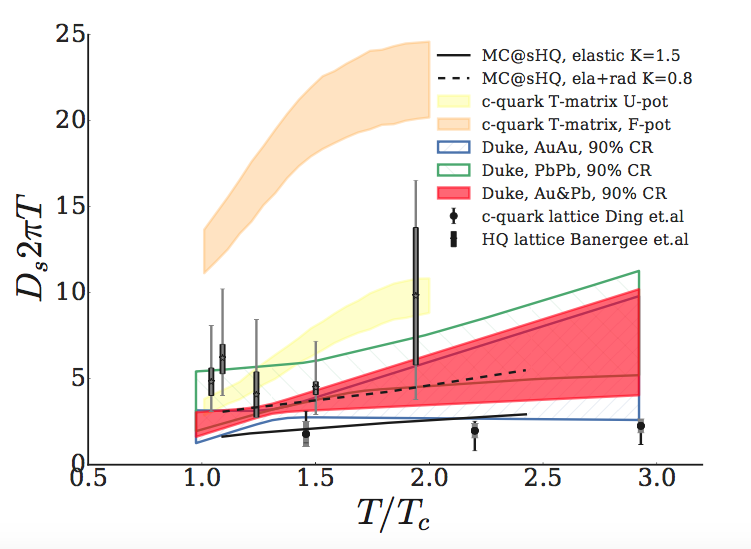
\includegraphics[width=10cm]{FigCap2/DiffCoeff.png}
  \caption{Estimated temperature dependence of the spatial diffusion coefficient  2$\pi T D_s(T/T_c)$, compared with other models calculations.}
  \label{fig:DiffCoeff}
\end{figure}

The larger data samples that will be collected during Run 3 and Run 4 at the LHC will
 allow to substantially reduce the measurement uncertainties, providing further constraints to models and
 constraining the values of the QGP transport coefficients.
